\begin{frame}
    \frametitle{Motivación}
    
    Las cámaras pueden ser utilizadas para realizar una reconstrucción del entorno y estimar la localización de un robot. Visual Odometry / Visual SLAM.
    
    \begin{center}
        \movie[showcontrols,autostart,loop,poster]{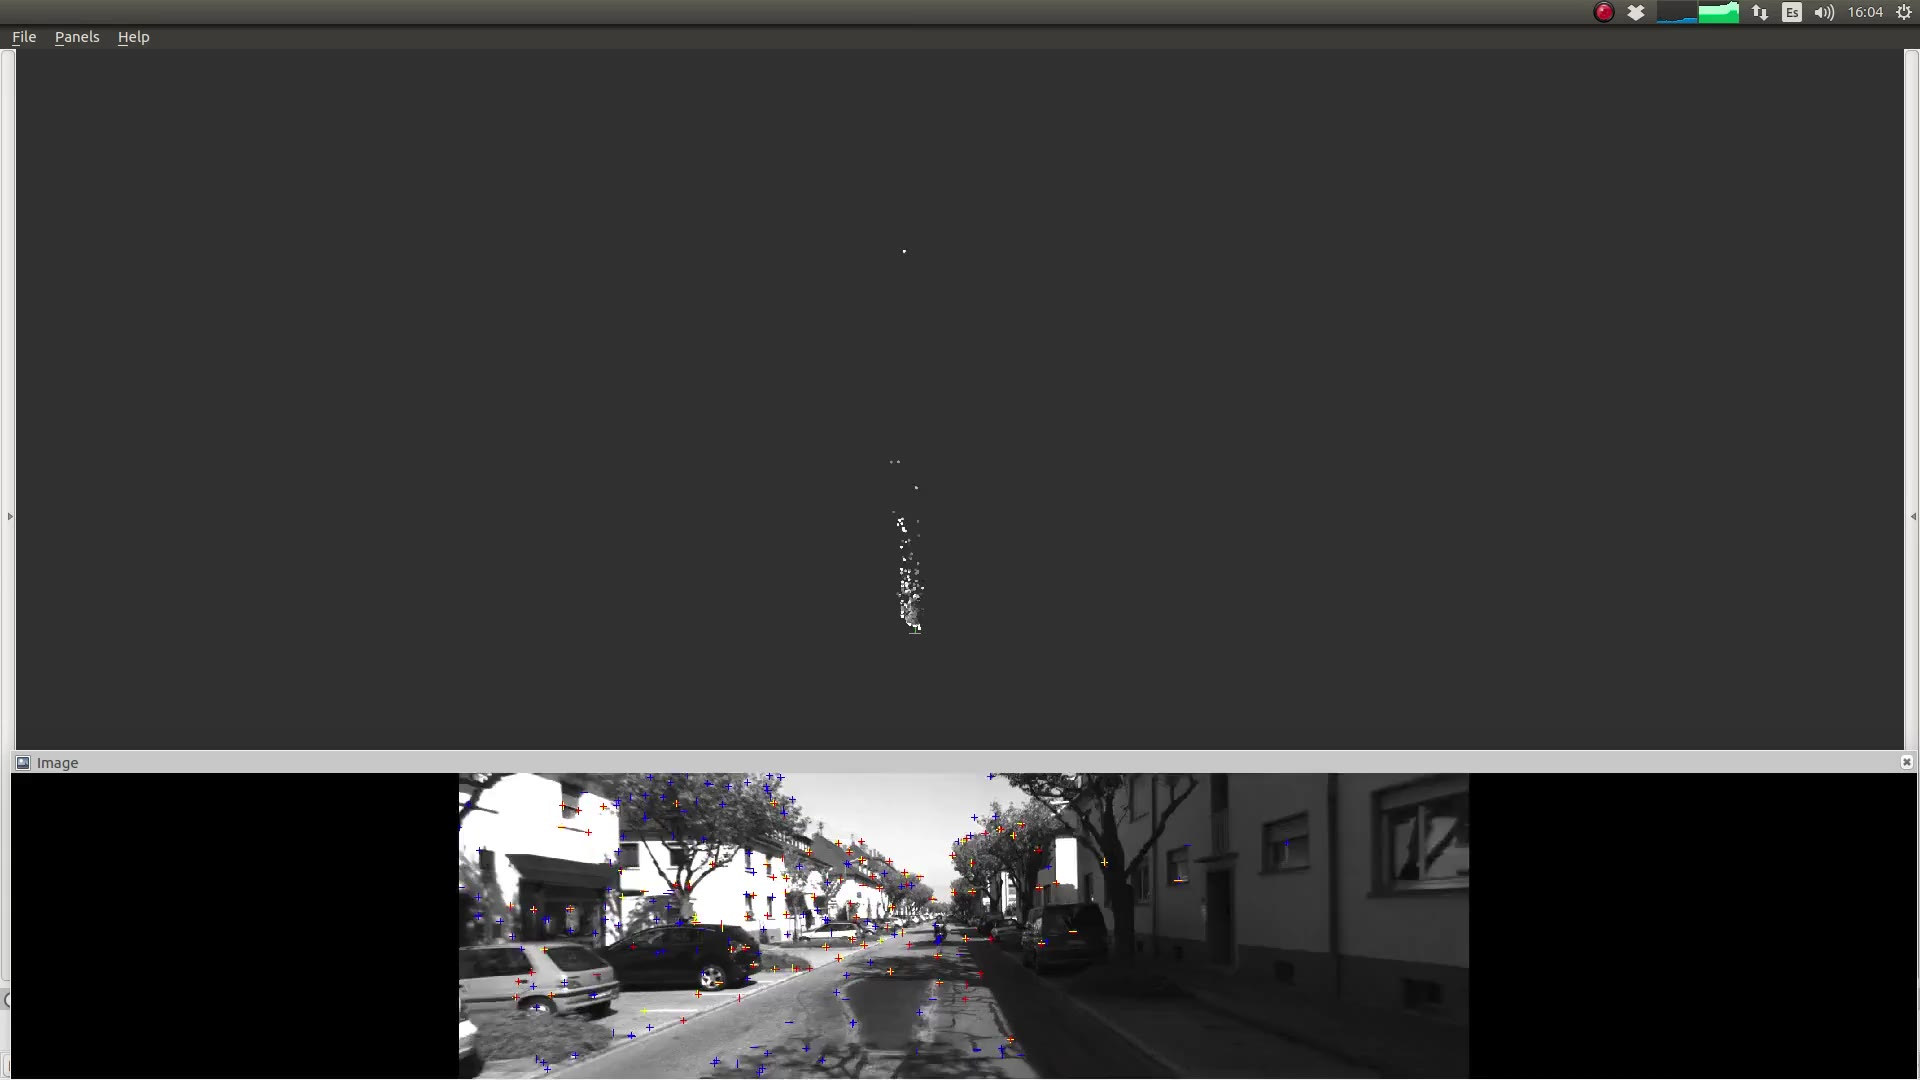
\includegraphics[width=0.75\columnwidth]{images/sptam_kitti_lc_trimmed_video.jpg}}{videos/sptam_kitti_lc_trimmed.mp4}
    \end{center}
    
\end{frame}

\begin{frame}
    \frametitle{Detección de Keypoints}
    
    \note{Slides fuertemente basadas de https://youtu.be/ebMyBbkkHWk}
    
    \note{https://3d.bk.tudelft.nl/courses/geo1016/slides/Lecture_03_Calibration.pdf}
    
    \footnotesize
    Propiedades deseables para SLAM / SfM:
    \begin{itemize}
        \item Alta repetitibilidad
        \item Invarianza (luminosidad, puntos de vista, etc)
        \item Computacionalmente eficientes
        \item Algunos detectores: HARRIS, SIFT, SURF, Shi-Tomasi, FAST, ORB, BRISK
    \end{itemize}

    
    \begin{figure}
        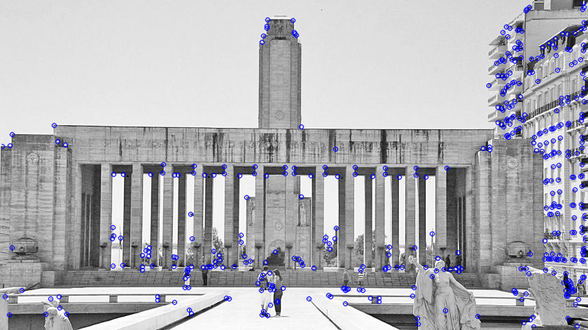
\includegraphics[width=0.5\textwidth]{./images/keypoints_fast}
        \caption{Keypoints FAST}
    \end{figure}

\end{frame}


\begin{frame}
    \frametitle{Matcheo de Keypoints}
    \footnotesize
    Propiedades deseables del matcheo de keypoints para SLAM / SfM:
    \begin{itemize}
        \item Alto recall
        \item Precisión
        \item Robustez
        \item Computacionalmente eficientes
        \item Posibles enfoques: patches o descriptores
    \end{itemize}
    
    \begin{figure}
        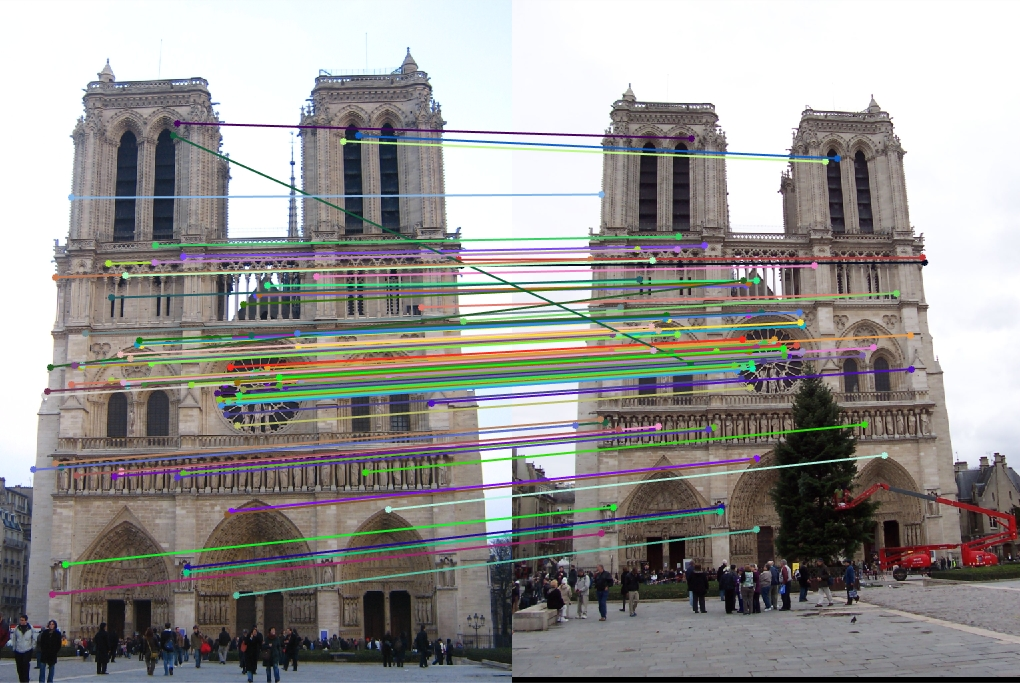
\includegraphics[width=0.4\textwidth]{./images/matching_notredam.jpg}
        \caption{Keypoints Harris + Descriptor SIFT}
    \end{figure}
    \note{Imagen extraida de https://www.cc.gatech.edu/classes/AY2016/cs4476_fall/results/proj2/html/cpolack6/index.html}
\end{frame}

\begin{frame}
    \frametitle{Precision - Recall}
    \footnotesize
    
    \note{https://upload.wikimedia.org/wikipedia/commons/2/26/Precisionrecall.svg}
    
    \begin{figure}
        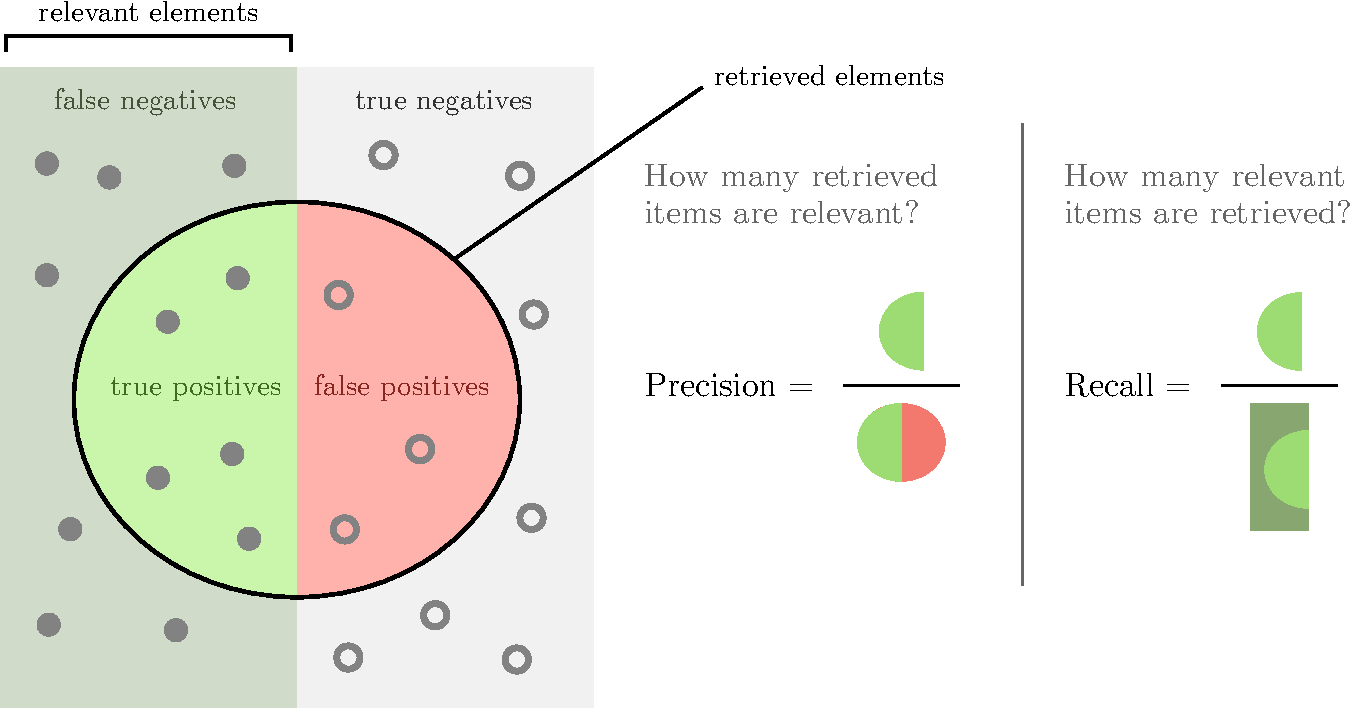
\includegraphics[width=0.9\textwidth]{./images/precision_recall.pdf}
    \end{figure}
\end{frame}

\begin{frame}
    \frametitle{Descriptores de Features Locales}
    \footnotesize
    
    Propiedades deseables para SLAM / SfM: distinguibles, robustos, invariantes
    \begin{itemize}
        \item Extraer firmas sobre regiones de la imagen, ejemplos:
        \begin{itemize}
            \item Histogramas sobre gradientes de la imagen (SIFT)
            \item Histogramas sobre respuestas Haar-wavelet (SURF)
            \item Patrones binarios (BRIEF, BRISK, FREAK, ORB)
            \item Descriptores basados en aprendizaje
        \end{itemize}
        \item Invariante rotación: Alineado con la orientación dominante de la región local
        \item Invariante a escala: Adaptar la región descripta a la escala de keypoint
    \end{itemize}

    \begin{figure}[!h]
        \subfloat[]
        {
            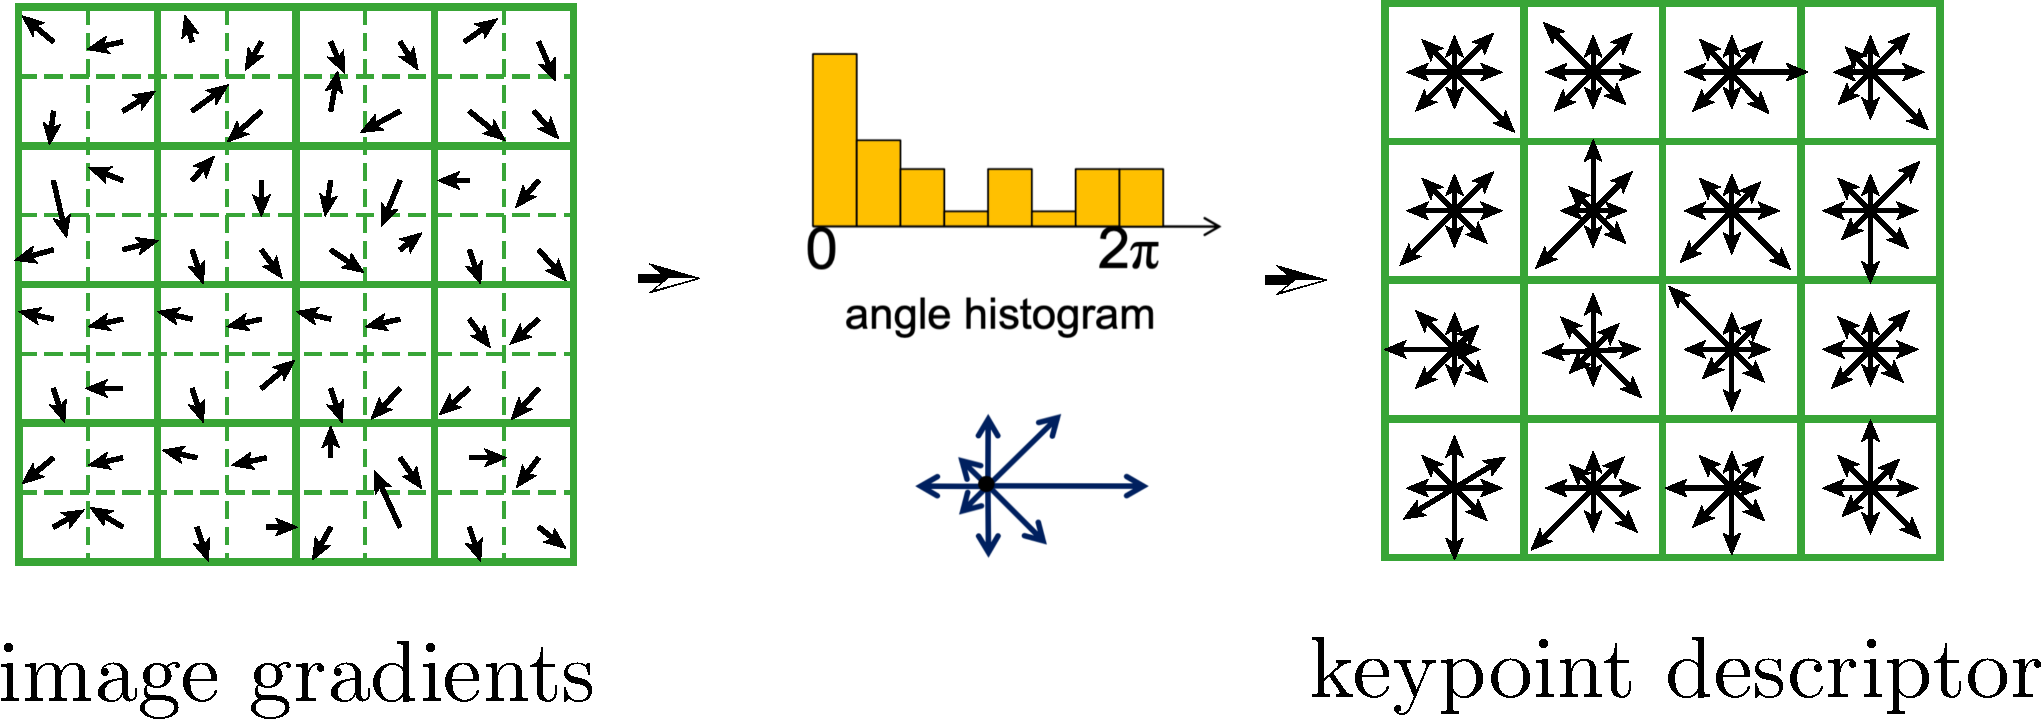
\includegraphics[width=0.6\columnwidth]{images/sift_gradient_pooling.pdf}
        }
        \hspace{1cm}
        \subfloat[]
        {
            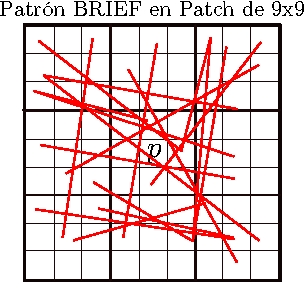
\includegraphics[width=0.3\columnwidth]{images/brief}
        }
    \end{figure}
    
\end{frame}

\begin{frame}
    \frametitle{Invarianza de Features Locales}
    \footnotesize
    
    \begin{itemize}
        \item Invarianza geométrica: traslación, rotación, escala.
        \item Invarianza fotométrica: brillo, exposición, etc.
    \end{itemize}
     

\end{frame}

\begin{frame}
    \frametitle{Ventajas de features locales}
    \footnotesize

    \begin{itemize}
    \item \textbf{Locales}: los features al ser locales son robustos a oclusiones
    \item \textbf{Distintivos}: pueden diferenciar un gran conjunto de objetos
    \item \textbf{Cuantiosos}: puede haber cientos o miles en una misma imagen
    \item \textbf{Eficientes}: al discretizar la imagen, se puede obtener tiempo real.
\end{itemize}
    
\end{frame}

\begin{frame}<presentation:0>[noframenumbering]
    \frametitle{Harris}
    \footnotesize
    
    \TODO{Agregar slides de SIFT, HARRIS, FAST y ORB \url{https://youtu.be/ebMyBbkkHWk}}
    
\end{frame}

\begin{frame}
    \frametitle{Características Visuales: Detector FAST}
    
    \begin{center}
        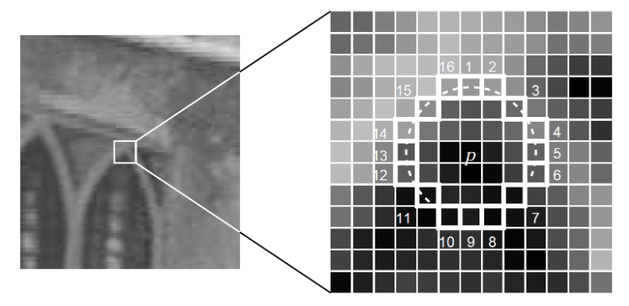
\includegraphics[width=0.7\textwidth]{./images/camera/fast}
    \end{center}
    
    \begin{itemize}
        \item El valor de intensidad del pixel $p$ es comparado con cada uno de los 16 pixeles del círculo de Bresenham alrededor de $p$.
        \item $p$ es detectado como corner si hay $12$ píxeles continuos en el circulo de Bresenham más brillosos u oscuros que $p$ dado un cierto umbral.
    \end{itemize}

\end{frame}

\begin{frame}
    \frametitle{Características Visuales: Descriptor BRIEF}
    \begin{minipage}[t]{0.35\columnwidth}
        \begin{figure}
            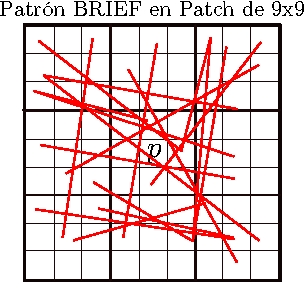
\includegraphics[width=\columnwidth]{./images/brief}
        \end{figure}
    \end{minipage}\hfill{}
    \begin{minipage}[t]{0.6\columnwidth}
        \centering
        256 Comparaciones entre píxeles (1 a 1)
        \begin{equation*}
            \tau(p;x,y) =
            \begin{cases}
                1 & \text{if $p(x) < p(y)$}\\
                0 & \text{otherwise}\\
            \end{cases}     
        \end{equation*}
        $s = \overbrace{01010010101110010...}^{256\ \text{bits}}$
    \end{minipage}
    \begin{block}{Matching distance}
        $\text{Hamming distance} = sum (XOR(s_{1}, s_{2}))$
    \end{block}
    \note{utilizamos la distancia de hamming para la distancia de matcheo entre descriptores.}
\end{frame}

\begin{frame}
    \frametitle{Extracción de features a diferentes escalas}
    
    \begin{figure}
        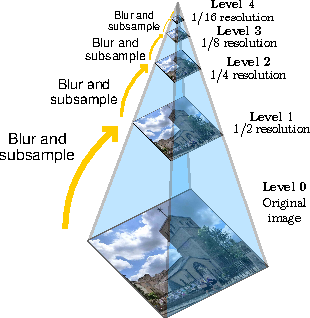
\includegraphics[width=0.5\textwidth]{./images/image_pyramid.pdf}
    \end{figure}

\end{frame}

\begin{frame}
    \frametitle{RANSAC: Random Sample Consensus}
    \footnotesize
    
    \begin{itemize}
        \item Permite encontrar un modelo que ajusta datos en presencia de ruido y outliers
        \item Separa el conjunto de datos entre inliers y outliers
%        \item Encuentra la mejor partición de puntos en un conjunto de inliers y outliers. Estima un modelo utilizando el conjunto de inliers.
        \item Ejemplo: dado un conjunto de puntos 2D, ajustar una línea 
    \end{itemize}
    
    \begin{figure}
        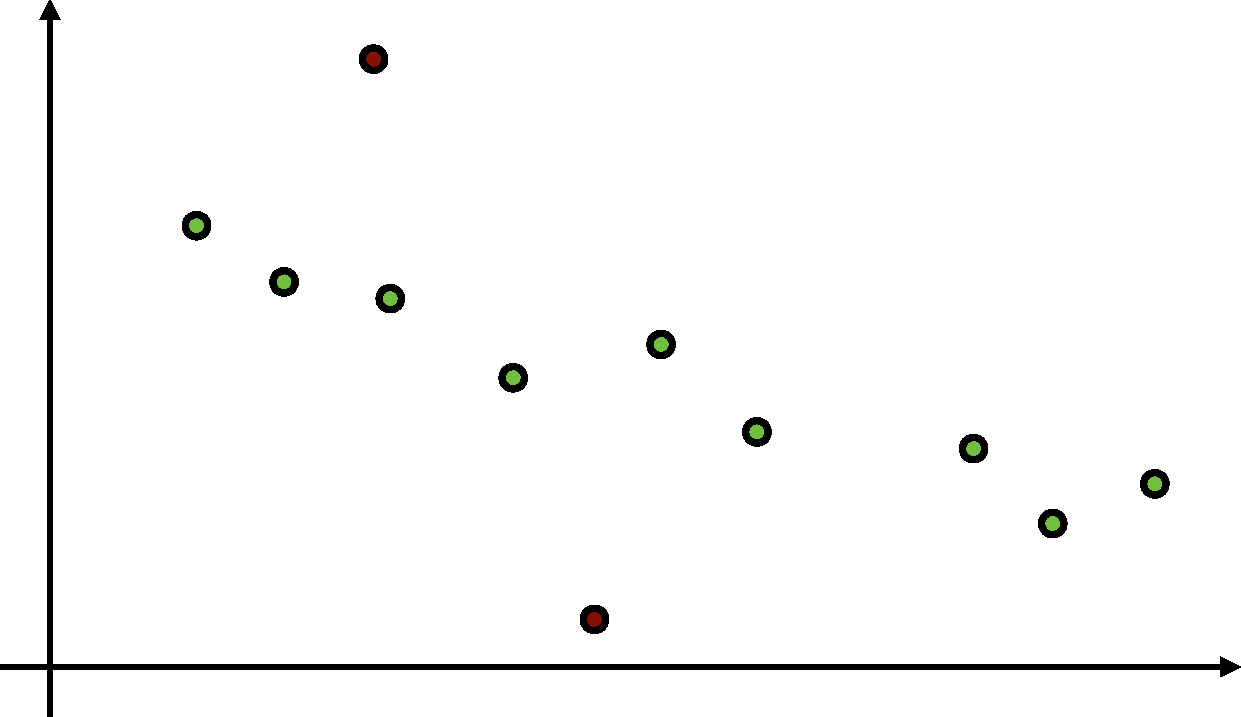
\includegraphics[width=0.5\textwidth]{./images/ransac1.pdf}
    \end{figure}
    
\end{frame}


\begin{frame}
    \frametitle{RANSAC: Random Sample Consensus}
    \footnotesize
    
    \only<1>{
        Podemos Ajustar una recta utilizando mínimos cuadrados, asumiendo ruido constante para todos los puntos
        \begin{figure}
            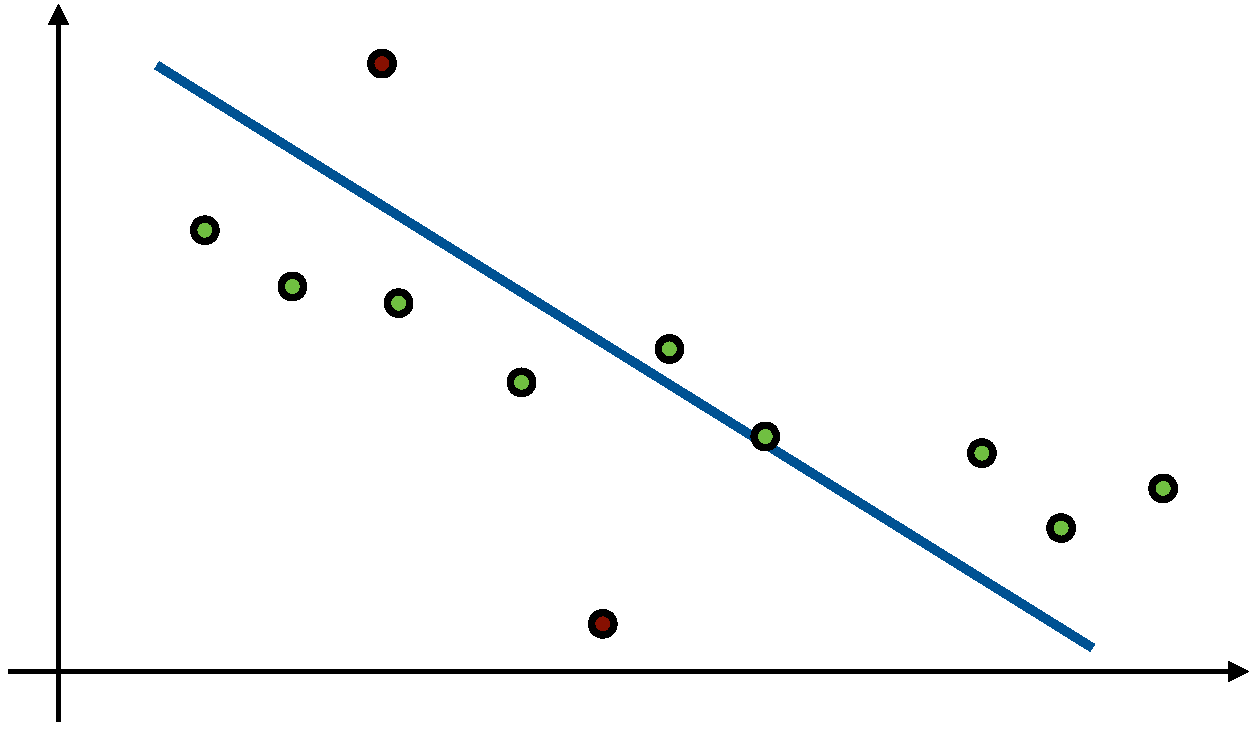
\includegraphics[width=0.5\textwidth]{./images/ransac2.pdf}
        \end{figure}
    }
    \only<2>{
           Podemos Ajustar una recta utilizando mínimos cuadrados, asumiendo ruido constante para todos los puntos
        \begin{figure}
            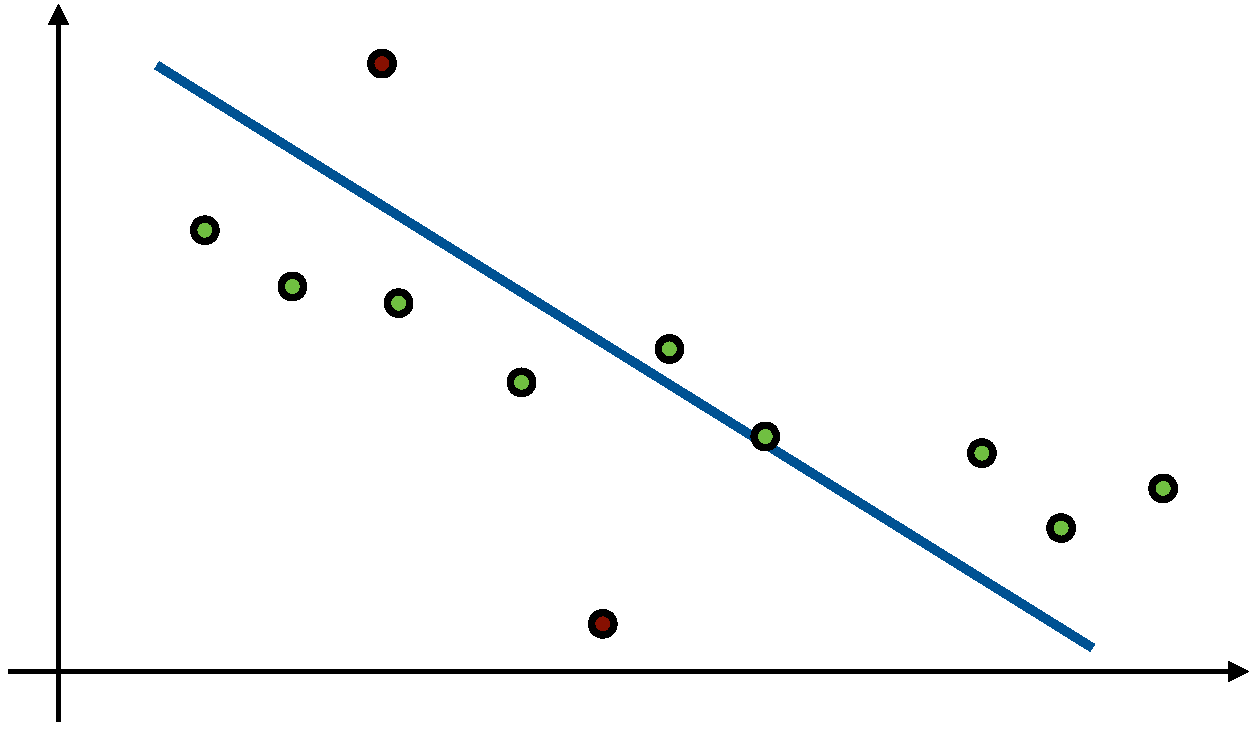
\includegraphics[width=0.5\textwidth]{./images/ransac2.pdf}
        \end{figure}
           Solo necesitamos 2 puntos para ajustar una recta!
        Probemos con 2 puntos aleatorios...
    }
    \only<3>{
        Probando con 2 puntos aleatorios
        \begin{figure}
            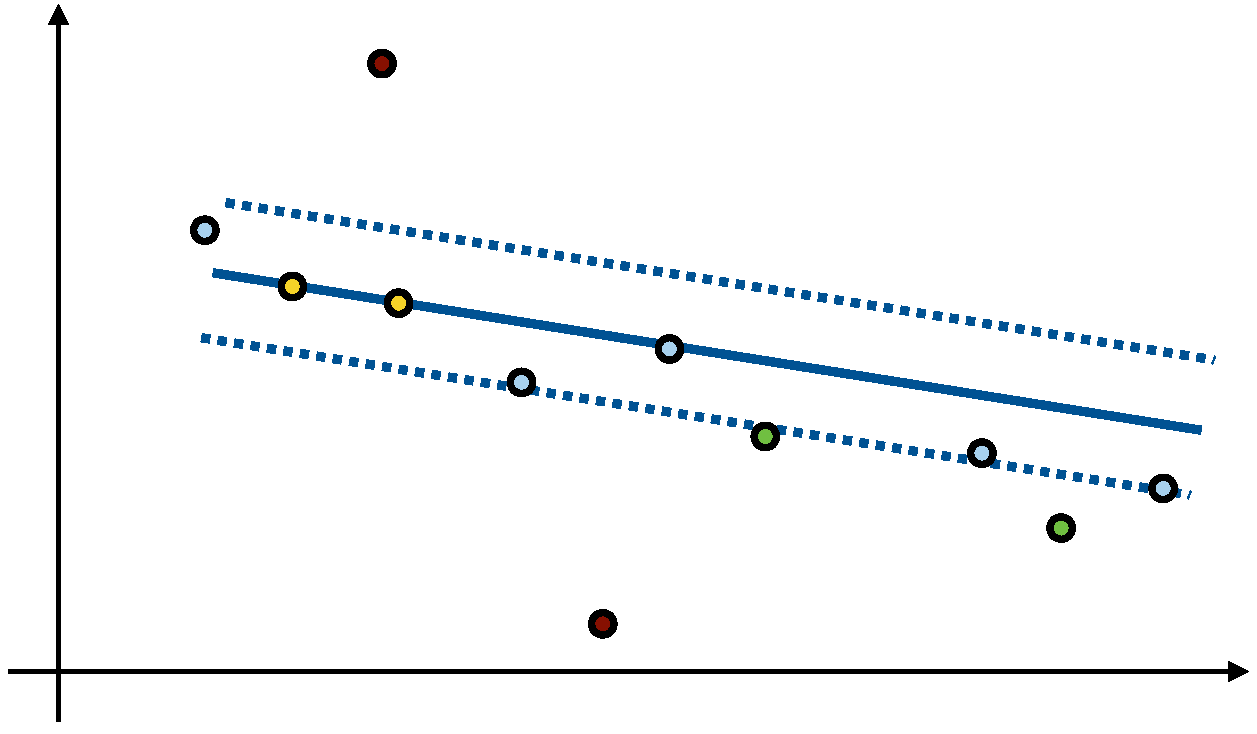
\includegraphics[width=0.5\textwidth]{./images/ransac3.pdf}
        \end{figure}
    }
    \only<4>{
        Probando con otros 2 puntos aleatorios
        \begin{figure}
            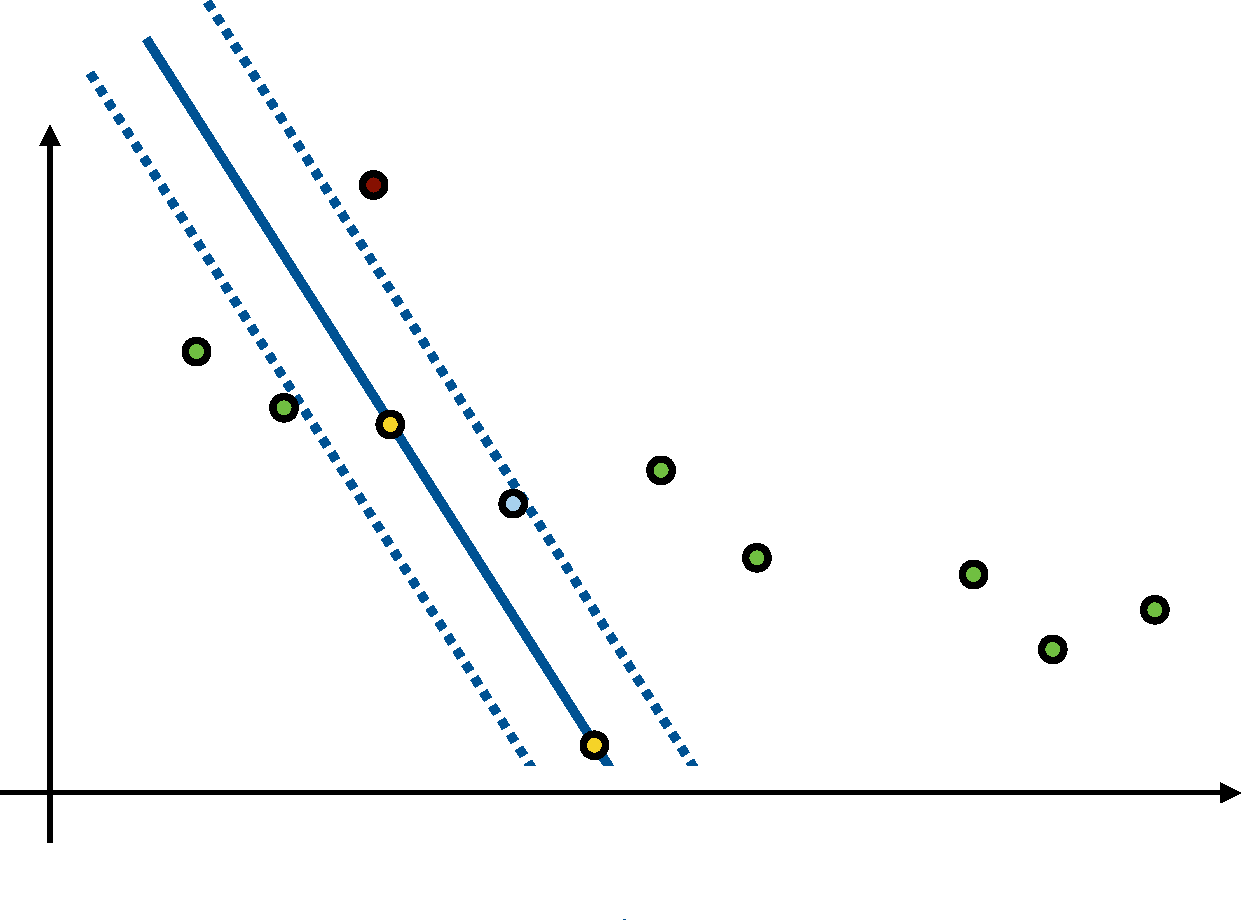
\includegraphics[width=0.5\textwidth]{./images/ransac4.pdf}
        \end{figure}
    }
    \only<5>{
        Probando con otros 2 puntos aleatorios
        \begin{figure}
            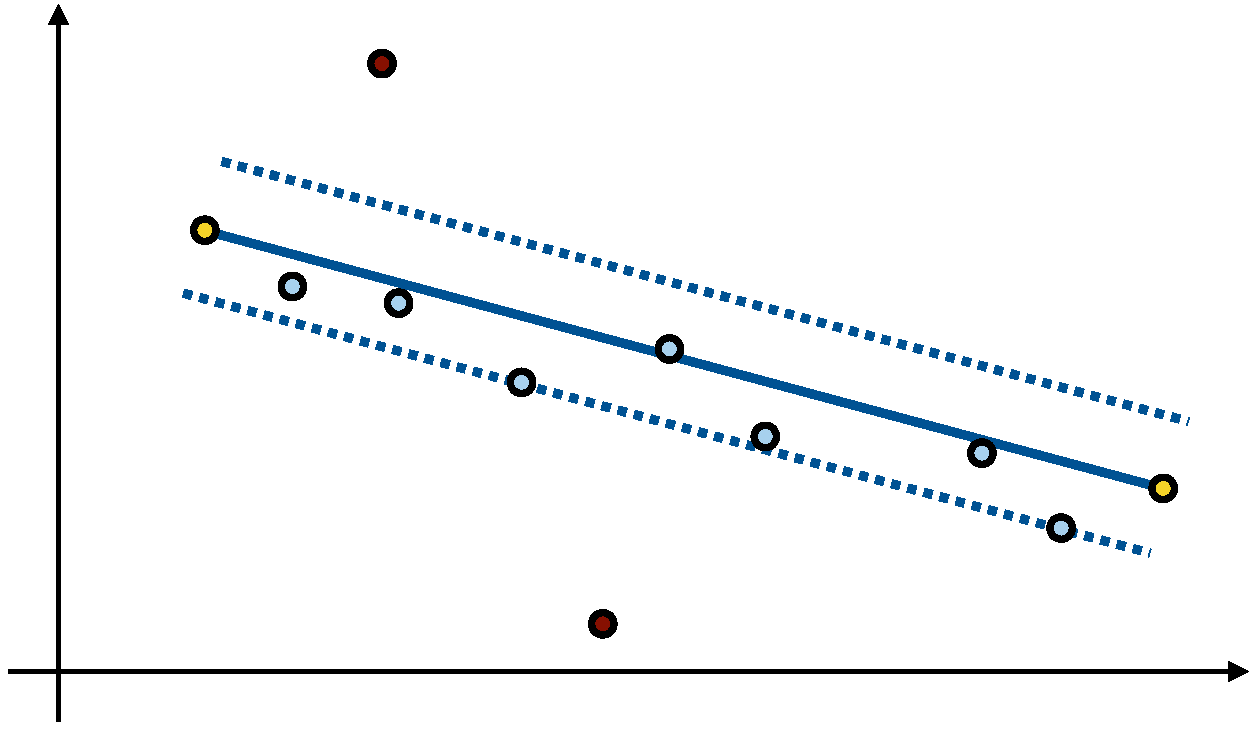
\includegraphics[width=0.5\textwidth]{./images/ransac5.pdf}
        \end{figure}
    }
    \only<6>{
        Utilicemos los inliers obtenidos con el mejor intento hasta ahora para realizar un ajuste con mínimos cuadrados
        \begin{figure}
            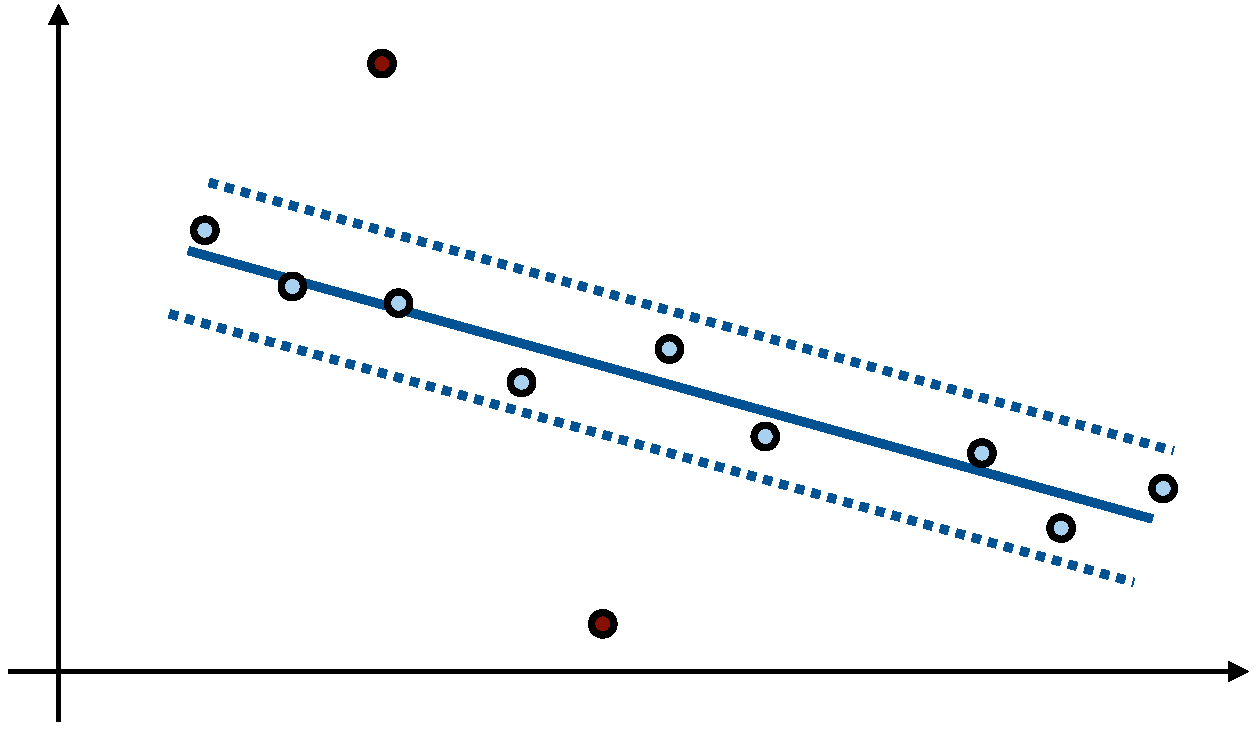
\includegraphics[width=0.5\textwidth]{./images/ransac6.pdf}
        \end{figure}
    }
\end{frame}


\begin{frame}
    \frametitle{RANSAC: Random Sample Consensus}
    \footnotesize

    \begin{enumerate}
        \item {\bf Samplear} de manera aleatoria el número de puntos requerido para ajustar el modelo.
        \item {\bf Computar} el modelo usando los datos sampleados
        \item {\bf Contar} el número de inliers y quedarse con el modelo que mejor ajusta los datos
        \item Iterar pasos 1-3 hasta que el mejor modelo es hallado
    \end{enumerate}

\end{frame}

\begin{frame}
    \frametitle{RANSAC: Random Sample Consensus}
    \footnotesize
    
    Pero...¿cuantas iteraciones realizar?
    
    \begin{itemize}
        \item Número de puntos sampleados $s$ (número de puntos mínimos requeridos para ajustar el modelo)
        \item Ratio de outliers $e = \dfrac{\# outliers}{\# puntos totales}$
        \item Número de intentos $T$.
        Elegimos $T$, con probabilidad $p$ de éxito (la probabilidad de al menos obtener un muestreo aleatorio libre de outliers en las $T$ iteraciones).
    \end{itemize}
    
    Probabilidad de fallar en una iteración, es decir de no seleccionar todos inliers.
    \begin{equation*}
        1-p = 1 - (1 - e)^{s}
    \end{equation*} 
    \note{(1-e)^s es la probabilidad de seleccionar todos inliers}
    
    
    Probabilidad de fallar en $T$ iteraciones, es decir seleccionar un outlier en todas las iteraciones.
    
    \begin{equation*}
        1-p = (1 - (1 - e)^{s})^{T}
    \end{equation*} 
    despejando $T$,
    \begin{equation*}
        T = \dfrac{\log(1-p)}{\log(1-(1-e)^{s})}
    \end{equation*} 
    
\end{frame}

\begin{frame}
    \frametitle{RANSAC: ventajas y desventajas}
    \footnotesize
    Ventajas:
    \begin{itemize}
        \item Robusto en presencia de outliers
        \item funciona bien para modelos de 1 a 10 parámetros (dependiendo del número de outliers)
        \item Fácil de implementar y entender
    \end{itemize}
    Desventajas:
    \begin{itemize}
        \item El tiempo computacional crece rápido con el porcentaje de outliers y el número de parámetros necesarios para ajustar el modelo
        \item No es bueno para obtener múltiples modelos (e.g. ajustar más de una línea en 2D)
    \end{itemize}
\end{frame}

\begin{frame}
    \frametitle{Cámara - Modelo Pin-Hole}
    
    \note{Ver libro de Sigwart. Seccion 4.2.3.2}
    \note{material sacado de mi tesis}
    
    \footnotesize
    \begin{figure}[!h]
        \subfloat[]
        {
            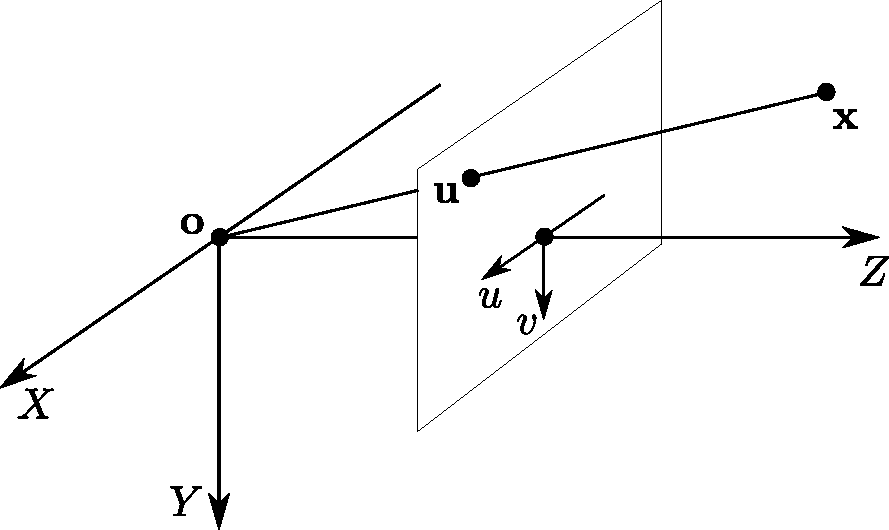
\includegraphics[width=0.28\columnwidth]{images/camera/pinhole_camera_model.pdf}
        }
        \subfloat[]
        {
            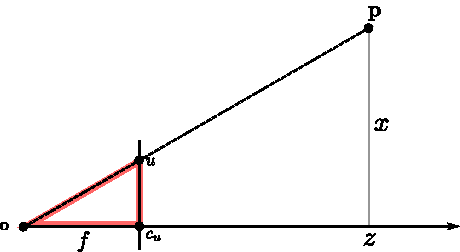
\includegraphics[width=0.28\columnwidth]{images/camera/pinhole_camera_model2.pdf}
        }
    \end{figure}
    
    \begin{block}{Modelo Pin-hole básico}
        Una Cámara permite obtener correspondencias entre el mundo 3D (espacio del objeto) y la imagen 2D. En el modelo de cámara pinhole, el punto de la imagen $\imagePoint=\begin{bmatrix}u & v\end{bmatrix}^{\top}$ se determina como la intersección entre el {\bf plano de la imagen} y el rayo que une el punto del mundo $\point =\begin{bmatrix}x & y & z\end{bmatrix}^{\top}$ y el {\bf centro de proyección óptico} $\cameraCenter$. 
    \end{block}
    
    \begin{itemize}
        \item $f$ es la \textbf{distancia focal}  (espcificada en \si{\milli\meter} o \si{\meter})
        \item $\principalPoint = \begin{bmatrix}0 & 0 & f\end{bmatrix}^{\top}$ es el \textbf{punto principal}
        \item el eje $Z$ es el {\bf eje principal}
        \item $\worldPoint$ es el punto en el sistema de coordenadas del mundo
    \end{itemize}
\end{frame}

\begin{frame}
    \frametitle{Cámara - Modelo Pin-Hole}
    
    \note{Ver libro de Sigwart. Seccion 4.2.3.2}
    \note{material sacado de mi tesis}
    
    \footnotesize
    \begin{figure}[!h]
        \centering
        \subfloat[]
        {
            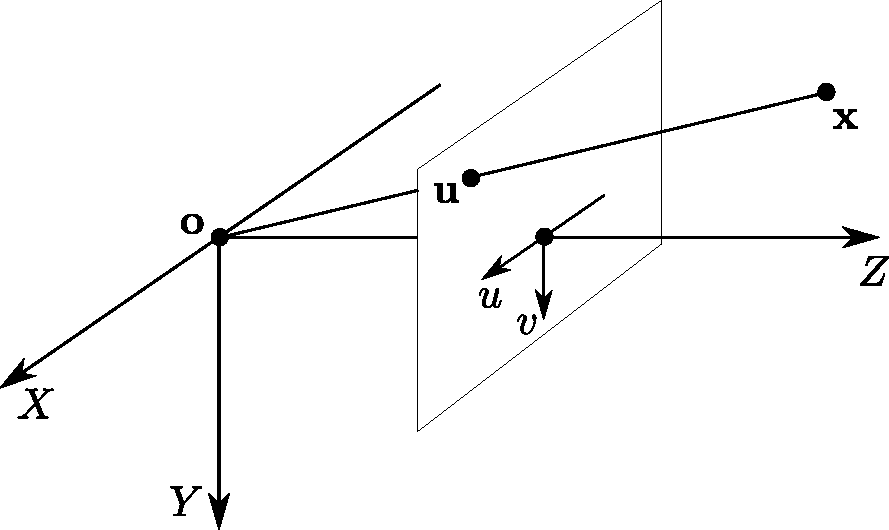
\includegraphics[width=0.3\columnwidth]{images/camera/pinhole_camera_model.pdf}
        }
        \subfloat[]
        {
            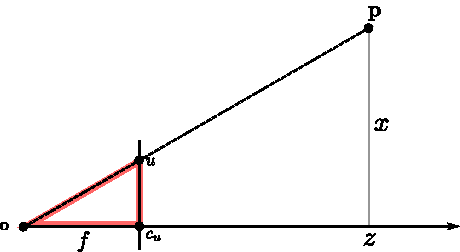
\includegraphics[width=0.3\columnwidth]{images/camera/pinhole_camera_model2.pdf}
        }
    \end{figure}
    
    \begin{itemize}
        \item El plano $Z = f$ se denomina {\bf plano principal} o {\bf plano de la imagen}.
        \item El punto en la imagen $\imagePoint=\begin{bmatrix}u & v\end{bmatrix}^{\top}$, en coordenadas 3D es $\imagePoint=\begin{bmatrix}x & y & f\end{bmatrix}^{\top}$
    \end{itemize}
\end{frame}


\begin{frame}
    \frametitle{Cámara - Modelo Pin-Hole}   
    \footnotesize
    \begin{figure}[!h]
        \centering
        \subfloat[]
        {
            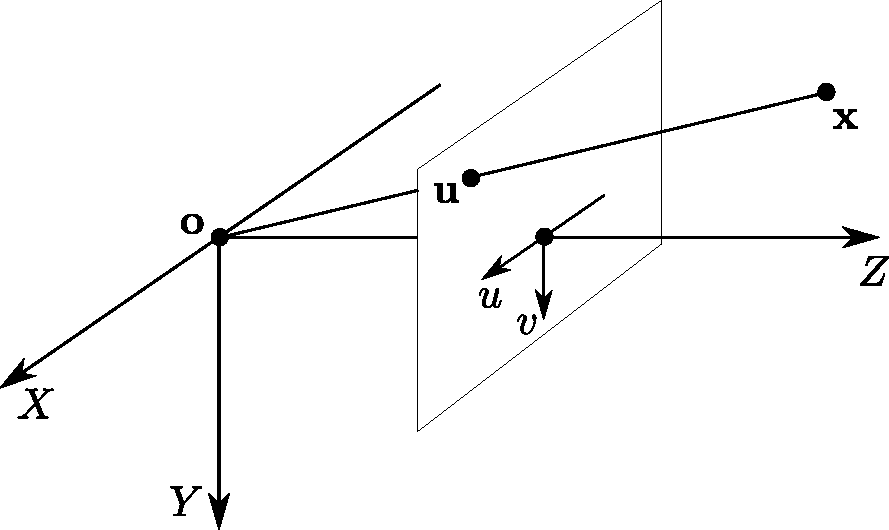
\includegraphics[width=0.3\columnwidth]{images/camera/pinhole_camera_model.pdf}
        }
        \subfloat[]
        {
            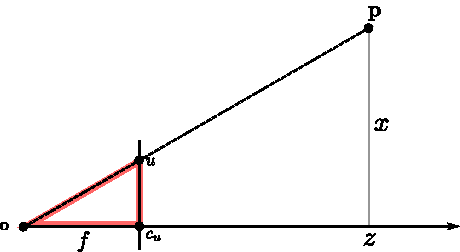
\includegraphics[width=0.3\columnwidth]{images/camera/pinhole_camera_model2.pdf}
        }
    \end{figure}

    Para obtener las coordenadas  $\imagePoint=\begin{bmatrix}u & v\end{bmatrix}^{\top}$ del punto $\worldPoint$ en el plano de la imagen, se proyecta $\worldPoint$ sobre el plano $ZX$ y $ZY$. Por similitud de triángulos para cada proyección:
    
    \begin{equation*}
        \dfrac{x}{z} = \dfrac{u}{f} \quad \text{y} \quad \dfrac{y}{z} = \dfrac{v}{f}
    \end{equation*}

    Por tanto, tenemos:
    
    \begin{equation*}
        u=\dfrac{fx}{z} \quad \text{y} \quad v=\dfrac{fy}{z}
    \end{equation*}
\end{frame}

\begin{frame}
    \frametitle{Cámara - Modelo Pin-Hole}   
    \footnotesize
    La correspondencia entre un punto $\mathbb{R}^{3}$ y $\mathbb{R}^{2}$ está dada por 
    
    \begin{equation*}
        \begin{bmatrix}x & y & z\end{bmatrix}^{\top} \rightarrow  \begin{bmatrix} u=\dfrac{fx}{z} & v=\dfrac{fy}{z} \end{bmatrix}^{\top}
    \end{equation*}

    Está correspondencia está dada por una transformación $\mathbb{P}^{3} \rightarrow \mathbb{P}^{2}$ tal que
    
    \begin{equation*}
        \projectionMatrix \homoWorldPoint= \homoImagePoint
    \end{equation*}
    donde $\projectionMatrix$ es la matríz asociada y se la denomina {\bf matríz de proyección}.
    
    \begin{equation}
        \begin{bmatrix}x & y & z\end{bmatrix}^{\top} \rightarrow  \begin{bmatrix} u=\dfrac{fx}{z} & v=\dfrac{fy}{z} \end{bmatrix}^{\top}
    \end{equation}

    Sea $\homoWorldPoint \in \mathbb{P}^{3}$, $\homoWorldPoint = \begin{bmatrix}x & y & z & 1\end{bmatrix}^{\top}$ entonces

    \begin{equation}
        \begin{bmatrix}
            fx\\
            fy\\
            z
        \end{bmatrix}
        =
        \begin{bmatrix}
            f & 0 & 0 & 0\\
            0 & f & 0 & 0\\
            0 & 0 & 1 & 0
        \end{bmatrix}
        \begin{bmatrix}
            x\\
            y\\
            z\\
            1
        \end{bmatrix}
    \end{equation}

\end{frame}

\begin{frame}
    \frametitle{Cámara - Modelo Pin-Hole}   
    \footnotesize
    
    \begin{figure}[!h]
        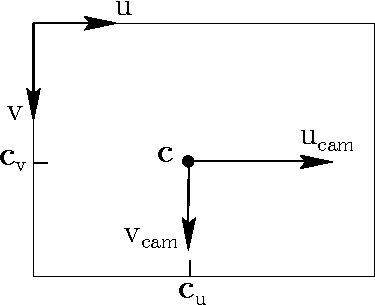
\includegraphics[width=0.2\columnwidth]{images/camera/principal_point_coordinates.pdf}
    \end{figure}

    \begin{itemize}
        \item El origen de coordenadas del plano de la imagen es el punto principal $\principalPoint = \begin{bmatrix}0 & 0 & f\end{bmatrix}^{\top}$
        \item Pero, el origen de coordenadas de la imagen digital es en la esquina superior izquierda. Por lo tanto, debemos aplicar una traslación, quedando:
    \end{itemize}
    

    %Como el origen de coordenadas del plano de la imagen (esquina superior izquierda) no coincide con el punto principal $\principalPoint = \begin{bmatrix}0 & 0 & f\end{bmatrix}^{\top}$, se aplica una traslación, quedando:
    
    \begin{equation}
        \begin{bmatrix}x & y & z\end{bmatrix}^{\top} \rightarrow  \begin{bmatrix} u=\dfrac{fx}{z} + \principalPoint_{u}& v=\dfrac{fy}{z} + \principalPoint_{v}\end{bmatrix}^{\top}
    \end{equation}

    Utilizando matrices
    \begin{equation}
    \begin{bmatrix}
        fx+z\principalPoint_{u}\\
        fy+z\principalPoint_{v}\\
        z
    \end{bmatrix}
    =
    \begin{bmatrix}
        f & 0 & \principalPoint_{u} & 0\\
        0 & f & \principalPoint_{v} & 0\\
        0 & 0 & 1 & 0
    \end{bmatrix}
    \begin{bmatrix}
        x\\
        y\\
        z\\
        1
    \end{bmatrix}
    \end{equation}
\end{frame}

\begin{frame}
    \frametitle{Cámara - Modelo Pin-Hole}   
    \footnotesize
    \begin{align*}
        \begin{bmatrix}
            fx+z\principalPoint_{u}\\
            fy+z\principalPoint_{v}\\
            z
        \end{bmatrix}
        &=
        \begin{bmatrix}
            f & 0 & \principalPoint_{u} & 0\\
            0 & f & \principalPoint_{v} & 0\\
            0 & 0 & 1 & 0
        \end{bmatrix}
        \begin{bmatrix}
            x\\
            y\\
            z\\
            1
        \end{bmatrix}\\
        \begin{bmatrix}
            fx+z\principalPoint_{u}\\
            fy+z\principalPoint_{v}\\
            z
        \end{bmatrix}
        &=
        \begin{bmatrix}f & 0 & \principalPoint_{u}\\
            0 & f & \principalPoint_{v}\\
            0 & 0 & 1
        \end{bmatrix}
        \begin{bmatrix}
            1 & 0 & 0 & 0\\
            0 & 1 & 0 & 0\\
            0 & 0 & 1 & 0
        \end{bmatrix}
        \begin{bmatrix}
            x\\
            y\\
            z\\
            1
        \end{bmatrix}
    \end{align*}
    Usando notación matricial, nos queda
    \begin{equation*}
        \underset{3 \times 4}{\projectionMatrix}=\underset{3 \times 3}{\intrinsicMatrix}\underset{3 \times 4}{\begin{bmatrix} \underset{3 \times 3}{\vec{I}} & \underset{3 \times 1}{\vec{0}}\end{bmatrix}},
    \end{equation*}
    donde $\intrinsicMatrix$ es la \textbf{matriz de calibración} o \textbf{matriz intrínseca}  de la cámara y está definida como,
    
    \begin{equation*}
        \intrinsicMatrix=
        \begin{bmatrix}f & 0 & \principalPoint_{u}\\
            0 & f & \principalPoint_{v}\\
            0 & 0 & 1
        \end{bmatrix}
    \end{equation*}
\end{frame}

\begin{frame}
    \frametitle{Cámara - Modelo Pin-Hole}
    
    \footnotesize
    
    \begin{figure}[!h]
        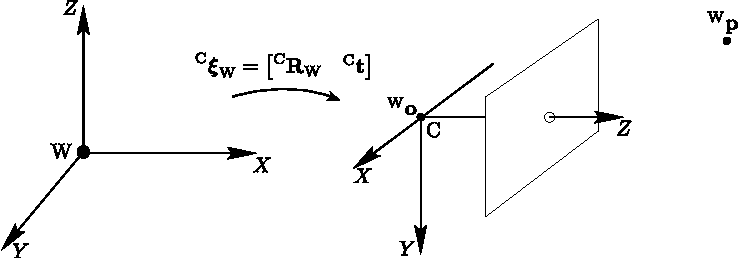
\includegraphics[width=0.6\columnwidth]{images/camera/camera_world_coordinate.pdf}
    \end{figure}
    
    En el caso general, la cámara no está ubicada en el centro del sistema de coordenadas del mundo. Tenemos que agregar esta transformación (rotación y traslación) entre el mundo y los sistemas de coordenadas de la cámara a la transformación.
    
    Dado el punto $\worldPoint$ en coordenadas del mundo $\worldCoordSystem$ , el mismo punto está descripto en el sistema de coordenadas de la cámara $\cameraCoordSystem$, y se lo representa $\cameraPoint$. Esto significa que $\cameraPoint$ está escrito en un sistema cuyo origen es $\worldCameraCenter$ y los ejes de de coordenadas sufrieron una rotación $\rotationCoord{\cameraCoordSystem}{\worldCoordSystem}$:
    
    \begin{equation*}
        \cameraPoint = \rotationCoord{\cameraCoordSystem}{\worldCoordSystem} \left( \worldPoint - \worldCameraCenter \right)
    \end{equation*}

\end{frame}

\begin{frame}
    \frametitle{Cámara - Modelo Pin-Hole}
    
    \footnotesize
    En coordenadsa homogeneas:
    \begin{equation*}
    \homoCameraPoint = 
    \begin{bmatrix}
            \cameraPoint\\
            1
    \end{bmatrix}=
    \begin{bmatrix}
    \left( \rotationCoord{\cameraCoordSystem}{\worldCoordSystem} \worldPoint -\rotationCoord{\cameraCoordSystem}{\worldCoordSystem} \worldCameraCenter \right)\\
    1
    \end{bmatrix} = 
    \begin{bmatrix}
        \rotationCoord{\cameraCoordSystem}{\worldCoordSystem} & -\rotationCoord{\cameraCoordSystem}{\worldCoordSystem} \worldCameraCenter \\
        \vec{0} & 1
    \end{bmatrix}
    \begin{bmatrix}
     \worldPoint\\
     1
    \end{bmatrix}
    \end{equation*}

    Reescribiendo $\translationCoord{\cameraCoordSystem}{\worldCoordSystem} = -\rotationCoord{\cameraCoordSystem}{\worldCoordSystem} \worldCameraCenter$
    
    \begin{equation*}
    \homoCameraPoint = 
    \begin{bmatrix}
            \cameraPoint\\
            1
    \end{bmatrix}= 
    \begin{bmatrix}
        \rotationCoord{\cameraCoordSystem}{\worldCoordSystem} & \translationCoord{\cameraCoordSystem}{\worldCoordSystem} \\
        \vec{0} & 1
    \end{bmatrix}
    \begin{bmatrix}
        \worldPoint\\
        1
    \end{bmatrix}
    \end{equation*}
    Luego si, $\homoImagePoint=\intrinsicMatrix\begin{bmatrix} \vec{I} & \vec{0}\end{bmatrix} \homoCameraPoint$ y $\homoCameraPoint =     \begin{bmatrix}
        \rotationCoord{\cameraCoordSystem}{\worldCoordSystem} & \translationCoord{\cameraCoordSystem}{\worldCoordSystem} \\
        \vec{0} & 1
    \end{bmatrix}
    \homoWorldPoint$, entonces
    
       \begin{equation*}
        \homoImagePoint=\intrinsicMatrix\begin{bmatrix} \vec{I} & \vec{0}\end{bmatrix} \begin{bmatrix}
            \rotationCoord{\cameraCoordSystem}{\worldCoordSystem} & \translationCoord{\cameraCoordSystem}{\worldCoordSystem} \\
            \vec{0} & 1
        \end{bmatrix}
        \homoWorldPoint
    \end{equation*}
    
    La matriz de proyección para el caso en que la cámara pueda ubicarse fuera del origen del mundo entonces queda:
    
    % \begin{equation*}
    %    \projectionMatrix=\intrinsicMatrix\begin{bmatrix}\rotationCoord{\cameraCoordSystem}{\worldCoordSystem} & \translationCoord{\cameraCoordSystem}{\worldCoordSystem}\end{bmatrix}
    % \end{equation*}

    \begin{center}
        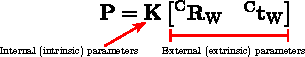
\includegraphics[width=0.4\columnwidth]{images/camera/projection_matrix.pdf}
    \end{center}

\end{frame}

\begin{frame}
    \frametitle{Cámara CCD}
    \footnotesize
    
    Los pixels del sensor CCD pueden no ser cuadrados. Si las coordenadas de la imagen son medidas en píxeles, entonces hay que tener en cuenta las dimensiones del pixel en cada dirección.
    
    \begin{figure}[!h]
        \centering
        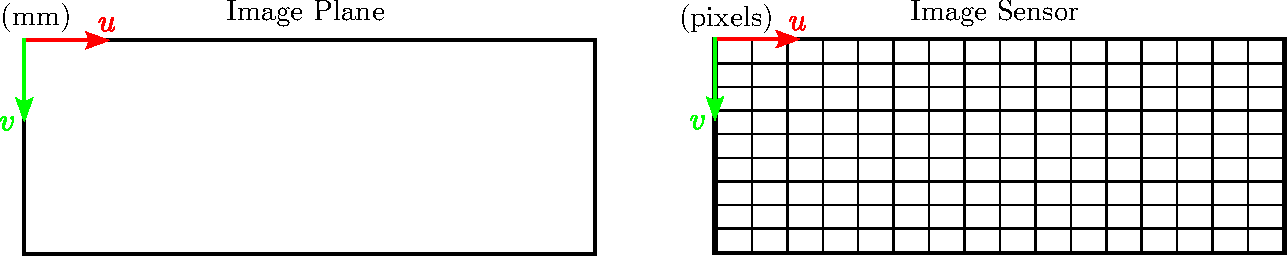
\includegraphics[width=0.6\columnwidth]{images/camera/rectangular_pixels.pdf}
    \end{figure}


    Sean
    \begin{itemize}
        \item $m_{u}$ : número de píxeles por milímetro (pixels/mm) en coordenadas de la
        imagen en la dirección $u$.
        \item $m_{v}$ : número de píxeles por milímetro (pixels/mm) en coordenadas de
        la imagen en la dirección $v$.
    \end{itemize}

    \begin{equation*}
        \intrinsicMatrix=
        \begin{bmatrix}f_{u} & 0 & \principalPoint_{u}\\
            0 & f_{v} & \principalPoint_{v}\\
            0 & 0 & 1
        \end{bmatrix},
    \end{equation*}

    donde $f_{u} = f m_{u} $ y $f_{v} = f m_{v}$ representan la distancia focal de la cámara en píxeles, en las direcciones $u$ e $v$ respectivamente.
\end{frame}

\begin{frame}
    \frametitle{Cámara proyectiva finita}
    \footnotesize
    
    Agregando más generalidad, puede ser que los píxeles estén ``torcidos'' debido a error de fabricación, aunque no es el caso usual.
    
    \begin{figure}[!h]
        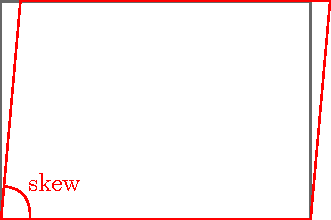
\includegraphics[width=0.3\columnwidth]{images/camera/pixel_skew.pdf}
    \end{figure}
    
    Para esto se agrega el parámetro \emph{skew} $s$ a la matriz de calibración
    
    \begin{equation*}
        \intrinsicMatrix=
        \begin{bmatrix}
            f_{u} & s & \principalPoint_{u}\\
            0 & f_{v} & \principalPoint_{v}\\
            0 & 0 & 1
        \end{bmatrix},
    \end{equation*}
    
\end{frame}

\begin{frame}
    \frametitle{Pin-hole camera model}
    
    El modelo de cámara Pin-Hole no modela la distorsión causada por los lentes.

    Las cámaras \emph{narrow} (FOV < 180 grados) utilizan coordenadas de píxeles $(x, y)$ o coordenadas de imagen normalizadas $(x_{n}, y_{n})$. 
    Las coordenadas de imagen normalizadas representan un vector 3D con la suposición implícita de que $z = 1$, lo que limita el FOV.

    Las cámaras \emph{wide} (sin límite de FOV, también conocidas como \emph{fisheye}) utilizan coordenadas esféricas $(x_{s}, y_{s}, z_{s})$, ya que no asumen que los puntos visibles siempre aparecen frente a la cámara.

    \begin{equation*}
        \begin{bmatrix}
            x\\
            y\\
            1
        \end{bmatrix} =
        \begin{bmatrix}
            f_{u} & s & \principalPoint_{u}\\
            0 & f_{v} & \principalPoint_{v}\\
            0 & 0 & 1
        \end{bmatrix}
        \begin{bmatrix}
            x_{n}\\
            y_{n}\\
            1
        \end{bmatrix}
    \end{equation*}
    
\end{frame}


\begin{frame}
    \frametitle{Distorsión Radial}
    
    \footnotesize
    
    Previamente, consideramos que el modelo de cámara pin-hole es perfectamente lineal, es decir, el punto en el mundo, el punto en la imagen y el centro óptico son colineales.
    
    Esta suposición no es cierta en la práctica porque hay una distorsión radial en la imagen producida por la lente de la cámara real.
    
    \begin{figure}[!h]
        \centering
        \subfloat[Sin distorsión]
        {
            
\includegraphics[width=0.2\columnwidth]{images/camera/no_distortion.pdf}
        }
        \subfloat[Barrel distortion]
        {
            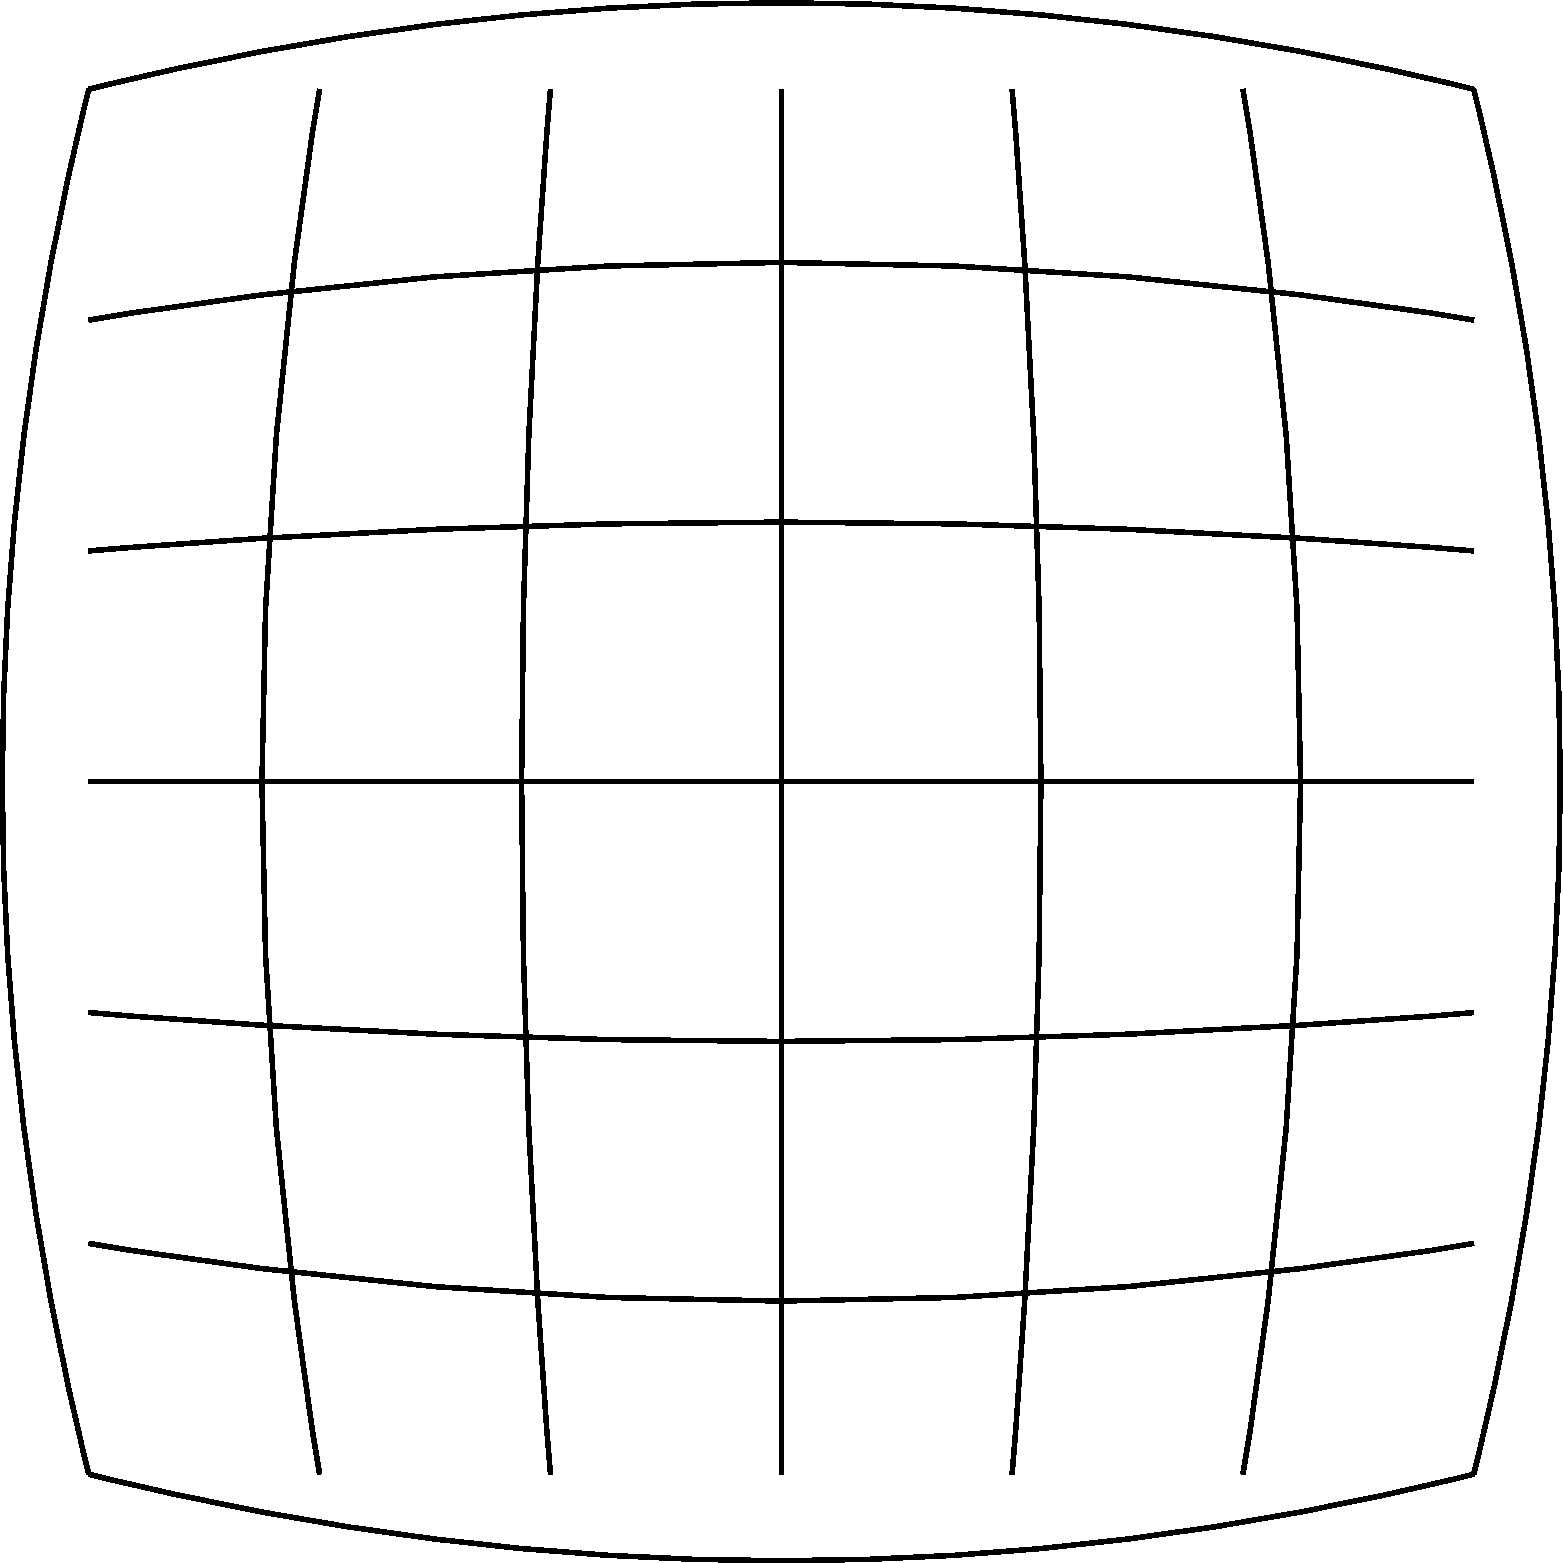
\includegraphics[width=0.2\columnwidth]{images/camera/barrel_distortion.pdf}
        }
        \subfloat[Pincushion distortion]
        {
            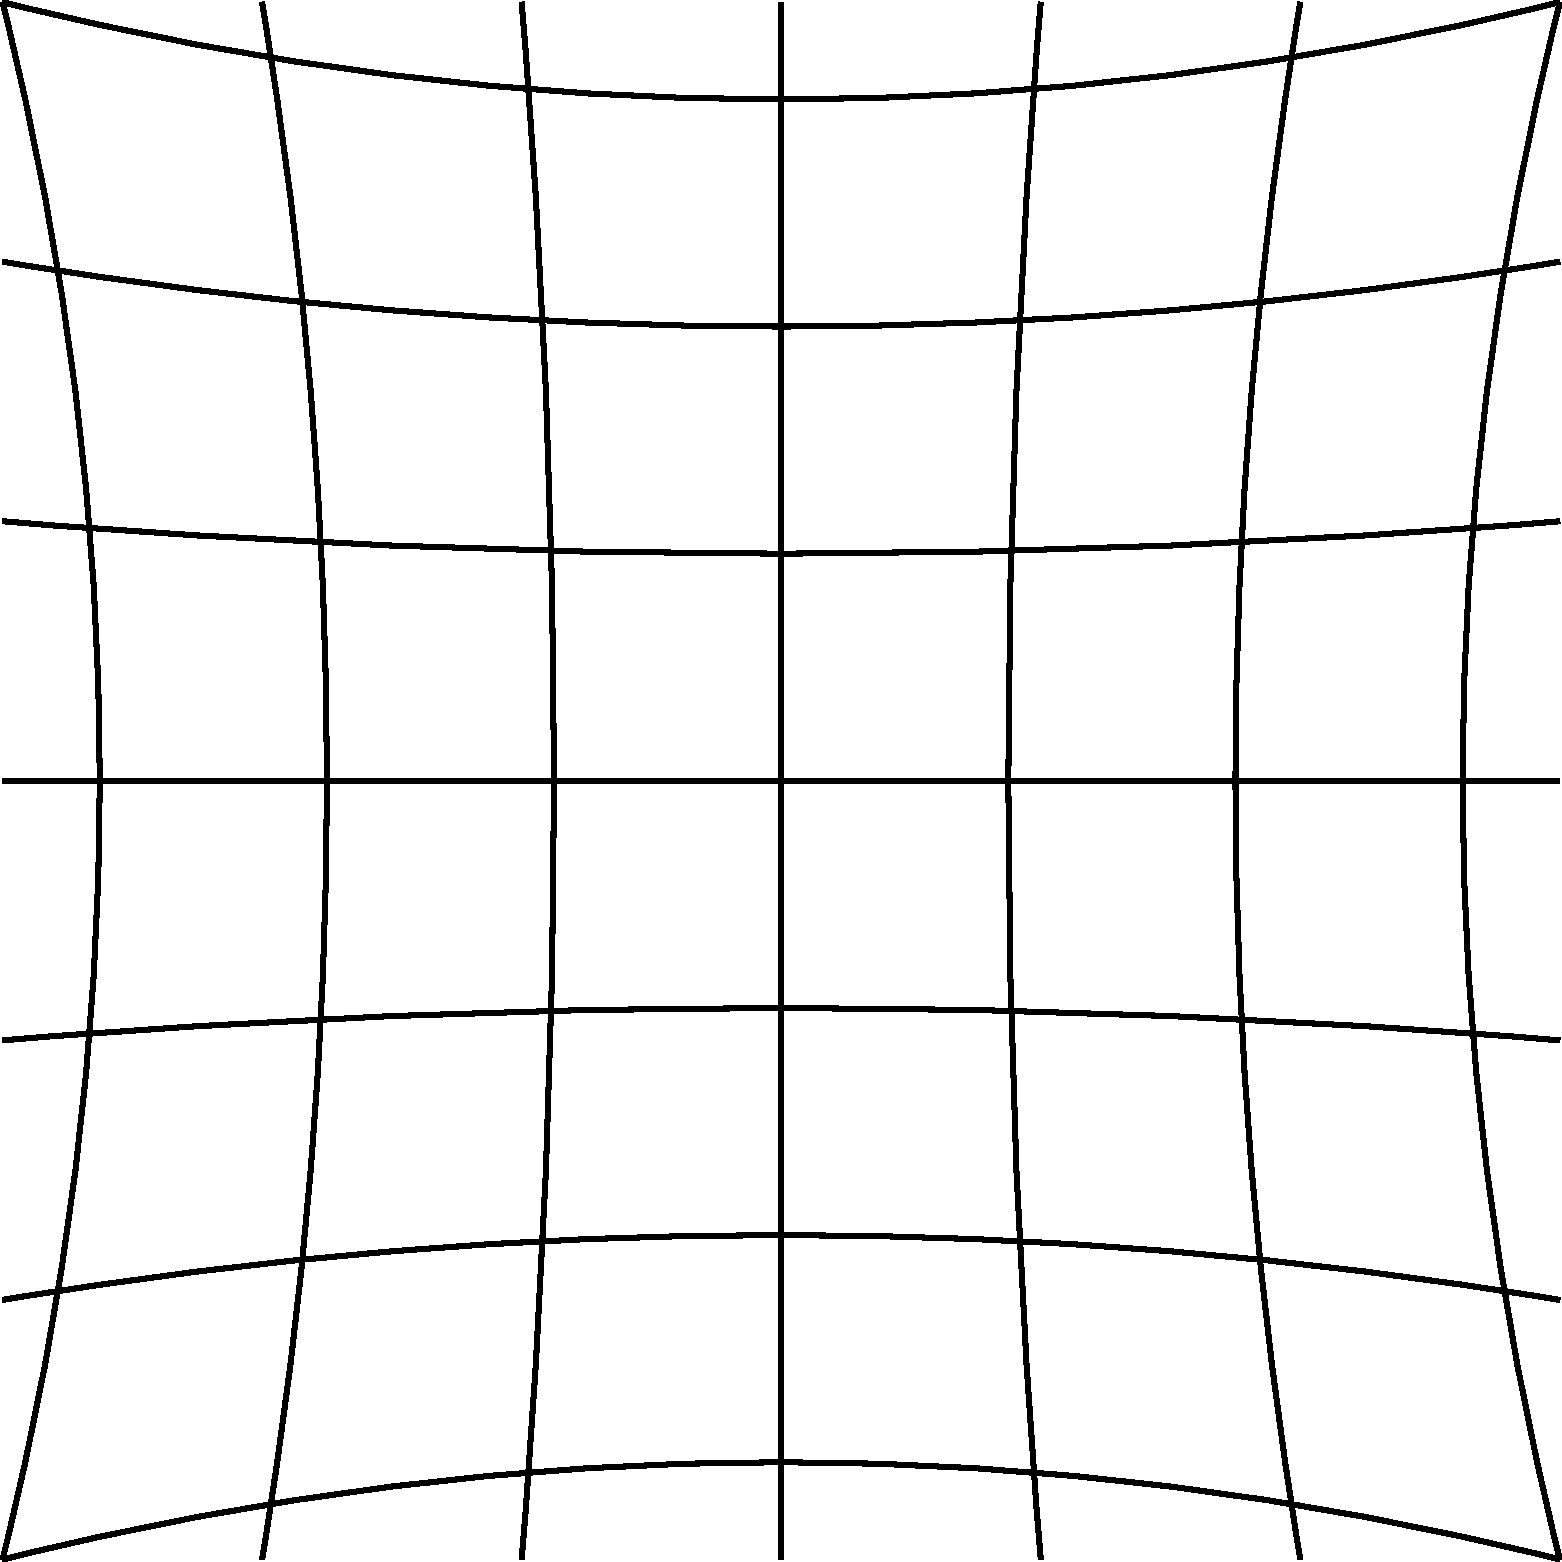
\includegraphics[width=0.2\columnwidth]{images/camera/pincushion_distortion.pdf}
        }
        \subfloat[Mustache distortion]
        {
            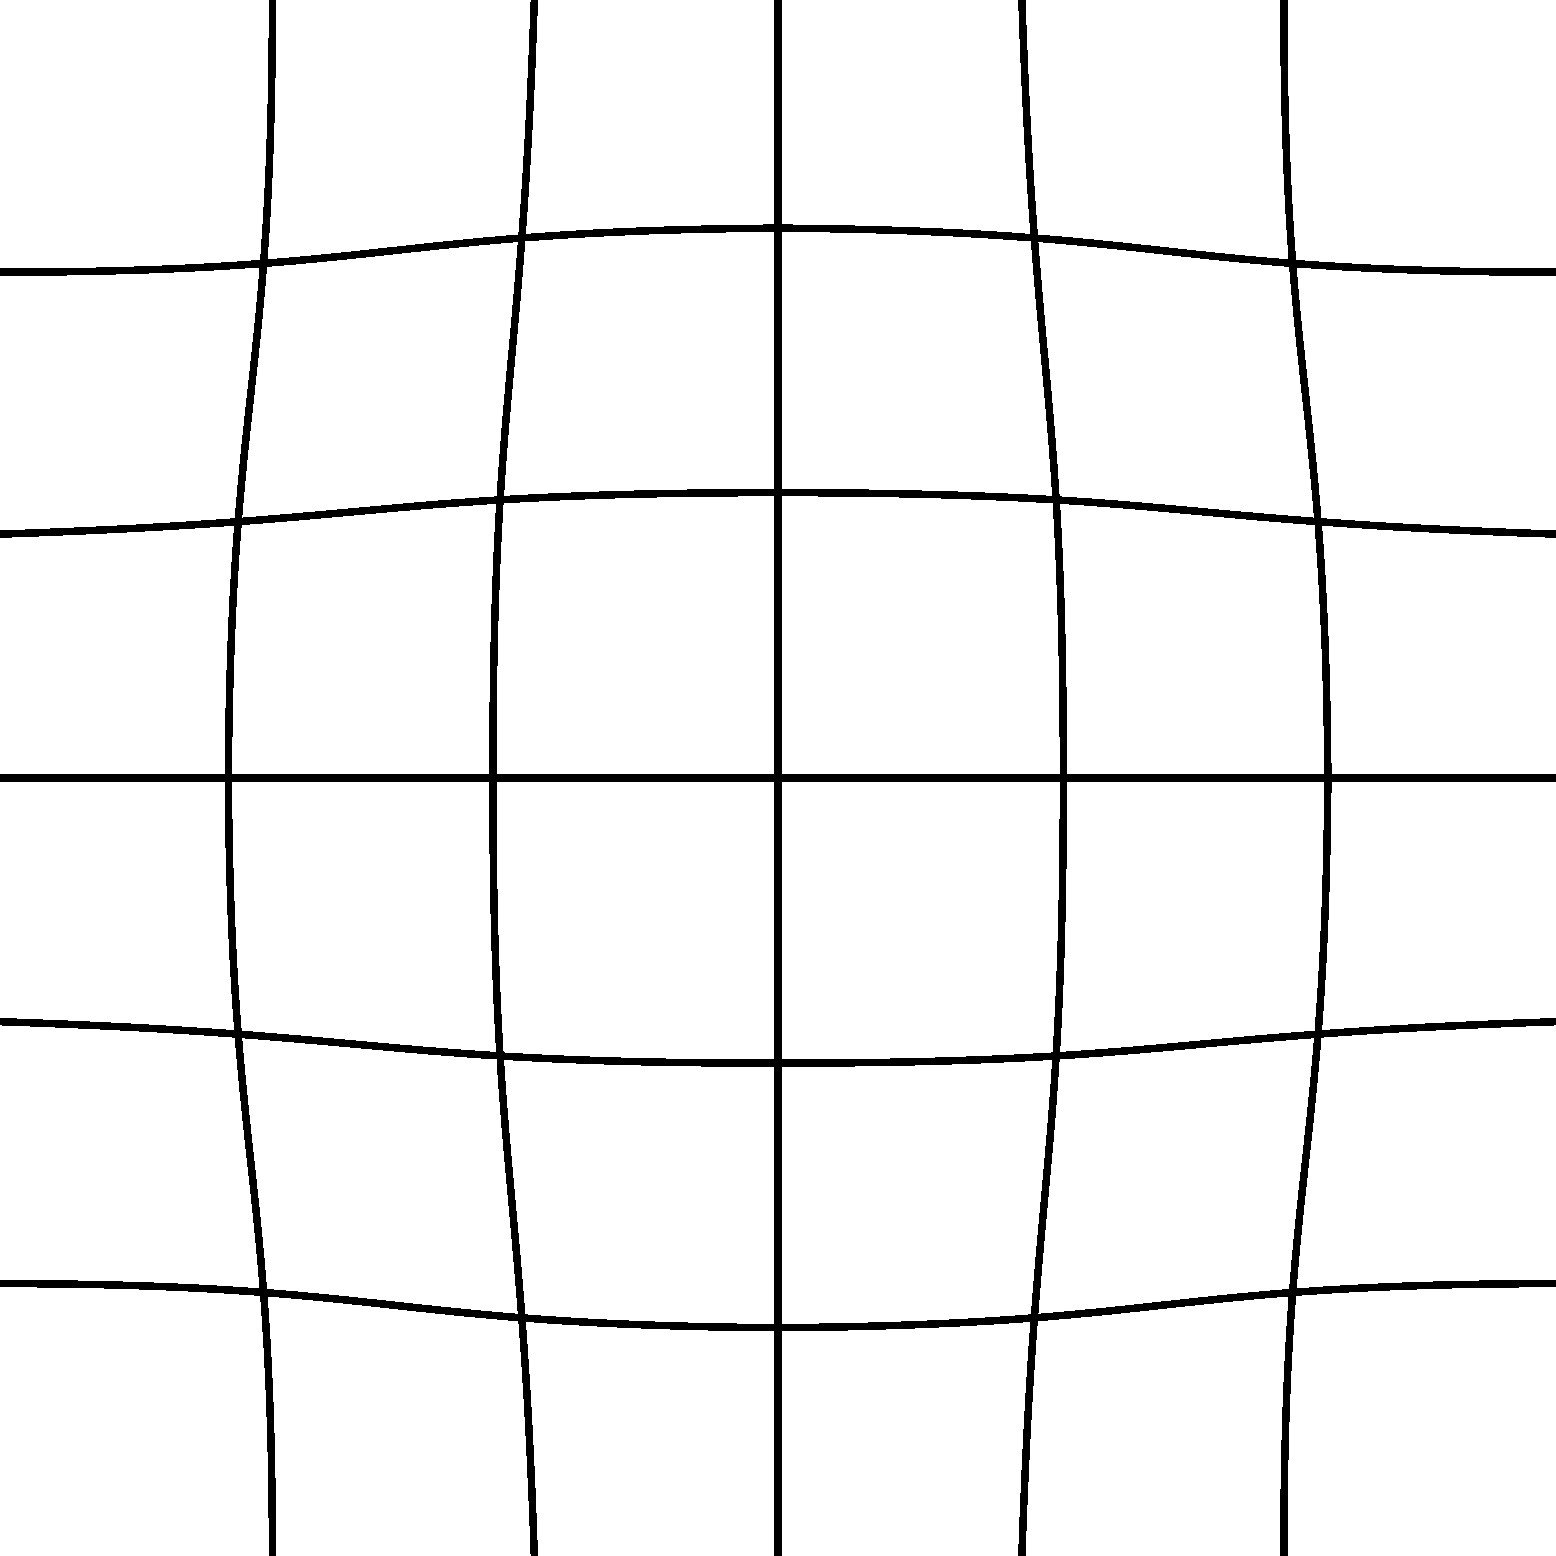
\includegraphics[width=0.2\columnwidth]{images/camera/mustache_distortion.pdf}
        }
    \end{figure}
    
\end{frame}

\begin{frame}
    \frametitle{Distorsión Radial}
    
    Para corregir esta distorsión se calcula un modelo de distorsión radial que relaciona los puntos de la imagen de la imagen real con los puntos ideales, los que se habrían obtenido bajo una cámara lineal perfecta. De esta forma, la cámara se puede representar con un modelo pin-hole lineal. En la figura es posible observar la imagen cruda (distorsionada) tomada por la cámara y la imagen después de la desdistorsión.
    
    \begin{figure}[!h]
        \centering
        \subfloat[Imagen distorsionada]
        {
            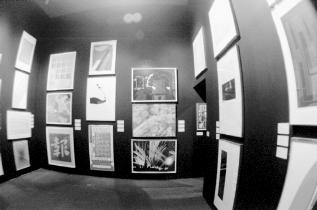
\includegraphics[width=0.45\columnwidth]{images/camera/distorted_image.png}
        }
        \subfloat[Imagen desdistorsionada]
        {
            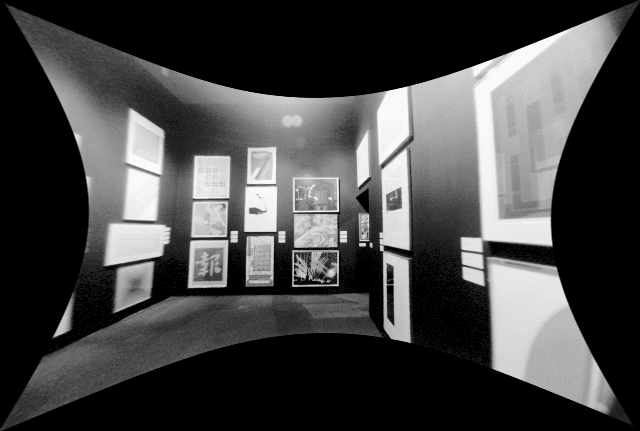
\includegraphics[width=0.45\columnwidth]{images/camera/undistorted_image.png}
        }
    \end{figure}
    
\end{frame}


% \begin{frame}
%     \frametitle{Distorsión Radial}
    
%     \footnotesize
    
%     Dado el punto proyectado real y el punto ideal, el efecto de distorsión radial se puede modelar mediante
%     \begin{equation}
%         \begin{bmatrix}u_{d}\\
%             v_{d}
%         \end{bmatrix}=L(\tilde{r})\begin{bmatrix}\tilde{u}\\
%             \tilde{v}
%         \end{bmatrix}
%     \end{equation}
    
%     donde, 
%     $\begin{bmatrix}\tilde{u}\\ 
%         \tilde{v}
%     \end{bmatrix}$
%     es la posición ideal de la imagen referida al centro de la imagen (que obedece a la proyección lineal);
%     $\begin{bmatrix}u_{d}\\
%         v_{d}
%     \end{bmatrix} $
%     es la posición real de la imagen después de la distorsión radial; $\tilde{r}$ es la distancia radial $\sqrt{\tilde{u}^{2}+\tilde{v}^{2}}$ desde el centro para la distorsión radial, y $L(\tilde{r})$ es una factor de distorsión, que es una función del radio $\tilde{r}$.
% \end{frame}

% \begin{frame}
%     \frametitle{Distorsión Radial}
%     \footnotesize
    
%     \TODO{Agregar modelo de distorsión aplicado en: https://boofcv.org/index.php?title=Tutorial\_Camera\_Calibration}
    
%     Finalmente, la corrección se puede representar en coordenadas de píxeles como
%     \begin{equation*}
%         \begin{aligned}\hat{u} & =u_{c}+L(r)(u-u_{c})\\
%             \hat{v} & =v_{c}+L(r)(v-v_{c})
%         \end{aligned}
%     \end{equation*}
    
%     donde 
%     $\begin{bmatrix}u\\
%         v
%     \end{bmatrix}$ 
%     son las coordenadas medidas, 
%     $\begin{bmatrix}\tilde{u}\\
%         \tilde{v}
%     \end{bmatrix}$ 
%     son las coordenadas corregidas, y 
%     $\begin{bmatrix}u_{c}\\
%         v_{c}
%     \end{bmatrix}$ 
%     es el centro de distorsión radial, con $r^{2}=(u-u_{c})^{2}+(v-v_{c})^{2}$.
    
%     El factor de distorsión $L(r)$ esta definido solo por valores positivos de $r$ y $L(0)=1$. En la práctica, $L(r)$ es aproximado por la expansión de Taylor
    
%     \begin{equation*}
%         L(r)=1+k_{1}r+k_{2}r^{2}+k_{3}r^{3}+\ldots.
%     \end{equation*}
    
%     Los coeficientes $\left\{ k_{1},k_{1},k_{1},\ldots,u_{c},v_{c}\right\}$ se consideran parte de la calibración interna de la cámara. Con frecuencia, el punto principal se utiliza como centro de la distorsión radial, aunque no es necesario que coincidan exactamente. Los coeficientes de corrección, junto con la matriz de calibración de la cámara, especifican el mapeo desde un punto de la imagen hasta un rayo en el sistema de coordenadas de la cámara y se denominan parámetros intrínsecos.
% \end{frame}

\begin{frame}
    \frametitle{Distorsión Tangencial}
    \footnotesize
    \begin{figure}
        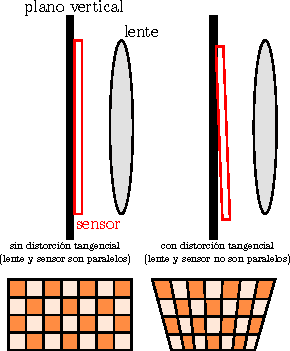
\includegraphics[width=0.4\columnwidth]{images/camera/tangential_distortion2.pdf}\\
    \end{figure}
    
\end{frame}

\begin{frame}
    \frametitle{Brown Camera Model}

    El modelo de cámara Brown es el más popular y modela la distorsión de la lente tanto por distorsión radial como por distorsión tangencial ("descentrante"). Es apropiado para la mayoría de lentes con un campo de visión menor a 180 grados.
    \begin{equation*}
        \begin{bmatrix}
            x \\
            y \\
            1
        \end{bmatrix} \approx K \begin{bmatrix}
            x_d \\
            y_d \\
            1
        \end{bmatrix}
    \end{equation*}
    \begin{equation*}
        \begin{bmatrix}
            x_d \\
            y_d
        \end{bmatrix} =
        \sum_{i=0}^{i<rad} k_{i} r^{2i}
        \begin{bmatrix}
            x_n \\
            y_n
        \end{bmatrix} +
        \begin{bmatrix}
            2p_{1} x_n y_n + p_{2} (r^2 + 2x_n^2) \\
            p_{1} (r^2 + 2y_n^2) + 2p_{2} x_n y_n
        \end{bmatrix}
    \end{equation*}
    donde $r = \sqrt{x_n^2 + y_n^2}$, $k_{i}$ son los coeficientes de distorsión radial y $(p_{1}, p_{2})$ son los coeficientes tangenciales.

    Los coeficientes $\left\{ k_{1}, k_{2}, k_{3}, \ldots , p_{1}, p_{2} \right\}$ se consideran parte de la calibración interna de la cámara. Con frecuencia, el punto principal se utiliza como centro de la distorsión radial, aunque no es necesario que coincidan exactamente. Los coeficientes de corrección, junto con la matriz de calibración de la cámara, especifican el mapeo desde un punto de la imagen hasta un rayo en el sistema de coordenadas de la cámara y se denominan parámetros intrínsecos.

    \note{Más info: https://boofcv.org/index.php?title=Tutorial\_Camera\_Calibration}
\end{frame}

\begin{frame}
    \frametitle{Kannala-Brandt Model}
    Kannala-Brandt es un modelo de cámara \emph{wide} que admite modelos de proyección en perspectiva, estereográfica, equidistante, de ángulo equisólido y ortogonal.

    \TODO{ver \url{https://docs.opencv.org/4.x/db/d58/group__calib3d__fisheye.html}}

    \note{Más info: https://boofcv.org/index.php?title=Tutorial\_Camera\_Calibration}
\end{frame}

\begin{frame}
    \frametitle{Calibración de cámara}
    \footnotesize
    
    \TODO{Ver Clase: Camera Calibration por Cyrill Stachniss: \url{https://www.youtube.com/watch?v=-9He7Nu3u8s}}

    \note{https://rpg.ifi.uzh.ch/docs/teaching/2025/03_camera_calibration.pdf}
    
\end{frame}


\begin{frame}
    \frametitle{Geometría Epipolar}

    \only<1>{
        \begin{center}
            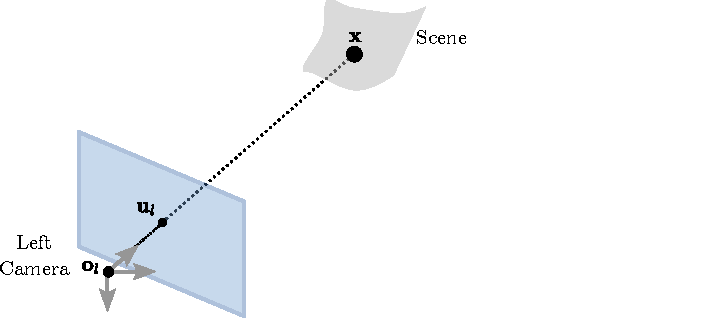
\includegraphics[width=0.6\textwidth]{./images/epipolar_geometry_monocular_left_observation.pdf}
        \end{center}
    }
    \only<2>{
        \begin{center}
            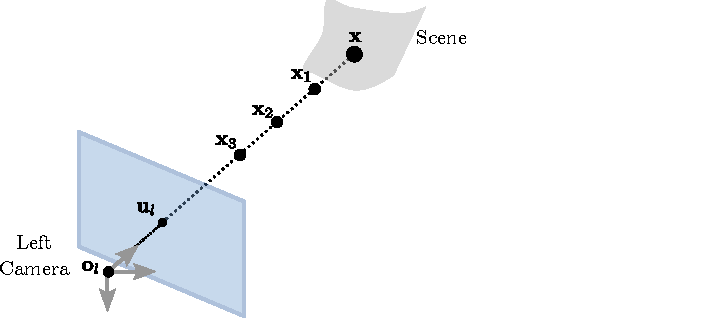
\includegraphics[width=0.6\textwidth]{./images/epipolar_geometry_monocular_left_observation_scale.pdf}
        \end{center}
    }
    \only<3>{
        \begin{center}
            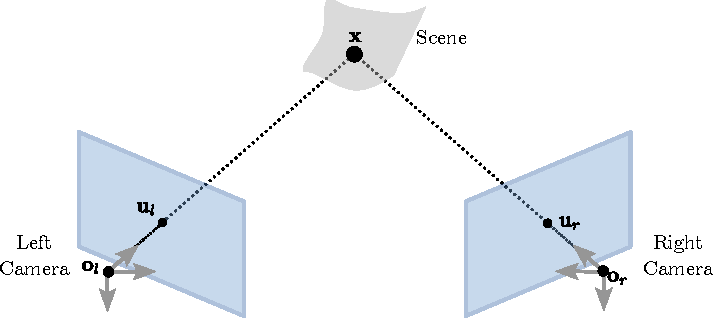
\includegraphics[width=0.6\textwidth]{./images/epipolar_geometry_monocular_stereo_observation.pdf}
        \end{center}
    }
    \only<4>{
        \begin{center}
            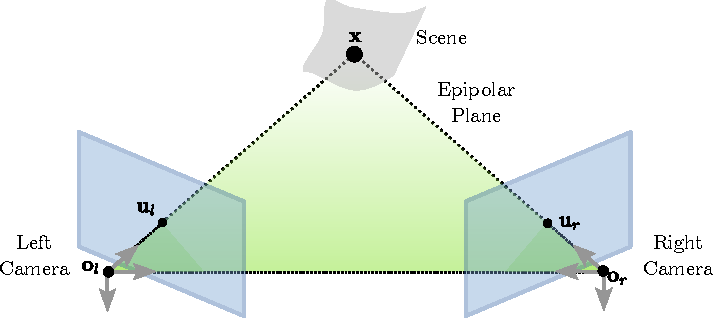
\includegraphics[width=0.6\textwidth]{./images/epipolar_geometry_epipolar_plane.pdf}
        \end{center}
    }
\end{frame}

% --- Slide 1: Epipolar Constraint (Geometric Basis) ---
\begin{frame}
    \frametitle{Epipolar Constraint}
    \begin{center}
        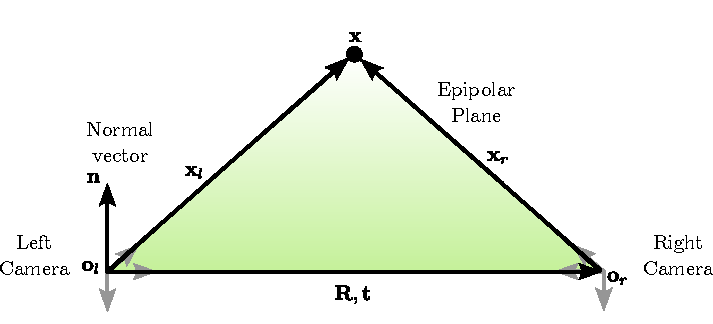
\includegraphics[width=0.6\textwidth]{./images/epipolar_geometry_normal_vector.pdf}
    \end{center}

    Vector normal to the epipolar plane: $\mathbf{n} = \translation \times \mathbf{x}_l$

    Dot product of $\mathbf{n}$ and $\mathbf{x}_l$ (perpendicular vectors) is zero:
    $$\boxed{\mathbf{x}_l \cdot (\translation \times \mathbf{x}_l) = 0}$$
\end{frame}

% --- Slide 2: Epipolar Constraint (Matrix Form) ---
\begin{frame}
    \frametitle{Epipolar Constraint}
    Writing the epipolar constraint in matrix form:
%
    \begin{equation*}
        \mathbf{x}_l \cdot (\translation \times \mathbf{x}_l) = 0
    \end{equation*}
%
    \begin{align*}
        \begin{bmatrix} x_l & y_l & z_l \end{bmatrix}
        \begin{bmatrix}
            t_y z_l - t_z y_l \\
            t_z x_l - t_x z_l \\
            t_x y_l - t_y x_l
        \end{bmatrix} &= 0 \quad \text{Cross-product definition}\\
        \begin{bmatrix} x_l & y_l & z_l \end{bmatrix}
        \underbrace{\begin{bmatrix}
            0 & -t_z & t_y \\
            t_z & 0 & -t_x \\
            -t_y & t_x & 0
        \end{bmatrix}}_{\begin{bmatrix}\translation\end{bmatrix}_{\times}}
        \begin{bmatrix} x_l \\ y_l \\ z_l \end{bmatrix} &= 0
        \quad \text{Matrix-vector form}
    \end{align*}
%
    \begin{equation*}
        \boxed{
        \mathbf{x}_l = \rotation \mathbf{x}_r + \translation
        }
        \quad
        \begin{bmatrix} x_l \\ y_l \\ z_l \end{bmatrix} =
        \begin{bmatrix}
            r_{11} & r_{12} & r_{13} \\
            r_{21} & r_{22} & r_{23} \\
            r_{31} & r_{32} & r_{33}
        \end{bmatrix}
        \begin{bmatrix} x_r \\ y_r \\ z_r \end{bmatrix} +
        \begin{bmatrix} t_x \\ t_y \\ t_z \end{bmatrix}
    \end{equation*}
\end{frame}

% --- Slide 3: Epipolar Constraint (Essential Matrix E) ---
\begin{frame}
    \frametitle{Epipolar Constraint}
    Substituting into the epipolar constraint gives:
    
    \begin{equation*}
        \begin{bmatrix} x_l & y_l & z_l \end{bmatrix}
        \left(
        \begin{bmatrix}
            0 & -t_z & t_y \\
            t_z & 0 & -t_x \\
            -t_y & t_x & 0
        \end{bmatrix}
        \begin{bmatrix}
            r_{11} & r_{12} & r_{13} \\
            r_{21} & r_{22} & r_{23} \\
            r_{31} & r_{32} & r_{33}
        \end{bmatrix}
        +
        \underbrace{
        \begin{bmatrix}
            0 & -t_z & t_y \\
            t_z & 0 & -t_x \\
            -t_y & t_x & 0
        \end{bmatrix}
        \begin{bmatrix} t_x \\ t_y \\ t_z \end{bmatrix}}_{\translation \times \translation = 0}
        \right)
        \begin{bmatrix} x_r \\ y_r \\ z_r \end{bmatrix} = 0
    \end{equation*}

    \begin{equation*}
        \begin{bmatrix} x_l & y_l & z_l \end{bmatrix}
        \underbrace{\begin{bmatrix}
            e_{11} & e_{12} & e_{13} \\
            e_{21} & e_{22} & e_{23} \\
            e_{31} & e_{32} & e_{33}
        \end{bmatrix}}_{\text{Essential Matrix } \essentialMatrix}
        \begin{bmatrix} x_r \\ y_r \\ z_r \end{bmatrix} = 0
    \end{equation*}

    \begin{equation*}
        \boxed{\essentialMatrix = \begin{bmatrix}\translation\end{bmatrix}_{\times} \rotation}
    \end{equation*}
    \footnotesize{[Longuet-Higgins 1981]}
\end{frame}

% --- Slide 4: Essential Matrix E Decomposition ---
\begin{frame}
    \frametitle{Essential Matrix $\essentialMatrix$: Decomposition}
    $$
    \boxed{\essentialMatrix = \begin{bmatrix}\translation\end{bmatrix}_{\times} \rotation}
    $$
    $$
    \begin{bmatrix}
        e_{11} & e_{12} & e_{13} \\
        e_{21} & e_{22} & e_{23} \\
        e_{31} & e_{32} & e_{33}
    \end{bmatrix} =
    \begin{bmatrix}
        0 & -t_z & t_y \\
        t_z & 0 & -t_x \\
        -t_y & t_x & 0
    \end{bmatrix}
    \begin{bmatrix}
        r_{11} & r_{12} & r_{13} \\
        r_{21} & r_{22} & r_{23} \\
        r_{31} & r_{32} & r_{33}
    \end{bmatrix}
    $$
    Given that $\begin{bmatrix}\translation\end{bmatrix}_{\times}$ is a Skew-Symmetric matrix ($a_{ij} = -a_{ji}$) and $\rotation$ is an Orthonormal matrix, it is possible to ``decouple'' $\translation_{\times}$ and $\rotation$ from their product using ``Singular Value Decomposition''.

    \vspace{0.5cm}
    Take Away: If $\essentialMatrix$ is known, we can calculate $\translation$ and $\rotation$.
\end{frame}




% --- Slide 5: How do we find E? ---
\begin{frame}
    \frametitle{How do we find $\essentialMatrix$?}
    Relates 3D position $(x_l, y_l, z_l)$ of scene point w.r.t left camera to its 3D position $(x_r, y_r, z_r)$ w.r.t. right camera
    \begin{equation*}
        \boxed{\mathbf{x}_l^{\top} \essentialMatrix \mathbf{x}_r = 0}
    \end{equation*}

    \begin{center}
        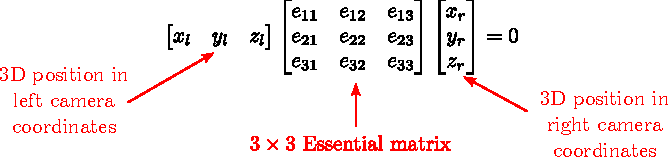
\includegraphics[width=0.8\textwidth]{./images/essential_matrix_coplanary_constraint.pdf}
    \end{center}

    Unfortunately, we don't have $\mathbf{x}_l$ and $\mathbf{x}_r$.

    But we do know corresponding points in image coordinates.
\end{frame}

\begin{frame}
    \frametitle{Incorporating the Image Coordinates}
    Perspective projection equations for left camera:
    \begin{align*}
        u_l &= f_u^{(l)} \frac{x_l}{z_l} + \principalPoint_{u}^{(l)} \quad & v_l &= f_v^{(l)} \frac{y_l}{z_l} + \principalPoint_{v}^{(l)} \\
        z_l u_l &= f_u^{(l)} x_l + z_l \principalPoint_{u}^{(l)} \quad & z_l v_l &= f_v^{(l)} y_l + z_l \principalPoint_{v}^{(l)}
    \end{align*}

    Representing in matrix form:
    \begin{equation*}
        z_l \begin{bmatrix} u_l \\ v_l \\ 1 \end{bmatrix} =
        \begin{bmatrix}
            z_l u_l \\
            z_l v_l \\
            z_l
        \end{bmatrix} =
        \begin{bmatrix}
            f_u^{(l)} x_l + z_l \principalPoint_{u}^{(l)} \\
            f_v^{(l)} y_l + z_l \principalPoint_{v}^{(l)} \\
            z_l
        \end{bmatrix} =
        \underbrace{\begin{bmatrix}
            f_u^{(l)} & 0 & \principalPoint_{u}^{(l)} \\
            0 & f_v^{(l)} & \principalPoint_{v}^{(l)} \\
            0 & 0 & 1
        \end{bmatrix}}_{\text{Known Camera Matrix } \intrinsicMatrix_l}
        \begin{bmatrix} x_l \\ y_l \\ z_l \end{bmatrix}
    \end{equation*}
\end{frame}

% --- Slide 6: Incorporating Image Coordinates (K) ---
\begin{frame}
    \frametitle{Incorporating the Image Coordinates}
    \begin{columns}[T]
        \begin{column}{0.5\textwidth}
            \centering
            \textbf{Left camera}
            \begin{align*}
                z_l \begin{bmatrix} u_l \\ v_l \\ 1 \end{bmatrix} &=
                \underbrace{\begin{bmatrix}
                    f_u^{(l)} & 0 & c_u^{(l)} \\
                    0 & f_v^{(l)} & c_v^{(l)} \\
                    0 & 0 & 1
                \end{bmatrix}}_{\intrinsicMatrix_{l}}\begin{bmatrix} x_l \\ y_l \\ z_l \end{bmatrix}\\
                z_{l} \begin{bmatrix} u_l \\ v_l \\ 1 \end{bmatrix} &= \intrinsicMatrix_{l} \vec{x}_{l}\\
                z_{l} \begin{bmatrix} u_l \\ v_l \\ 1 \end{bmatrix}^{\top} &= \vec{x}_{l}^{\top} \intrinsicMatrix_{l}^{\top}
            \end{align*}
        \end{column}
        \begin{column}{0.5\textwidth}
            \centering
            \textbf{Right camera}
            \begin{align*}
                z_r \begin{bmatrix} u_r \\ v_r \\ 1 \end{bmatrix} &=
                \underbrace{\begin{bmatrix}
                    f_u^{(r)} & 0 & c_u^{(r)} \\
                    0 & f_v^{(r)} & c_v^{(r)} \\
                    0 & 0 & 1
                \end{bmatrix}}_{\intrinsicMatrix_r}
                \begin{bmatrix} x_r \\ y_r \\ z_r \end{bmatrix}
            \end{align*}
        \end{column}
    \end{columns}
    \vspace*{-0.5em}
    \begin{equation*}
        \boxed{
            \mathbf{x}_l^{\top} = \begin{bmatrix} u_l & v_l & 1 \end{bmatrix} z_l \intrinsicMatrix_l^{-\top}
        }
        \quad
        \boxed{
        \mathbf{x}_r = \intrinsicMatrix_r^{-1} z_r \begin{bmatrix} u_r \\ v_r \\ 1 \end{bmatrix}
        }
    \end{equation*}
\end{frame}

% --- Slide 7: Incorporating Image Coordinates (Substitution) ---
\begin{frame}
    \frametitle{Incorporating the Image Coordinates}
    %
    Epipolar constraint:
    %
    \begin{equation*}
        \begin{bmatrix} x_l & y_l & z_l \end{bmatrix}
        \begin{bmatrix}
            e_{11} & e_{12} & e_{13} \\
            e_{21} & e_{22} & e_{23} \\
            e_{31} & e_{32} & e_{33}
        \end{bmatrix}
        \begin{bmatrix} x_r \\ y_r \\ z_r \end{bmatrix} = 0
    \end{equation*}
    %
    Rewriting in terms of image coordinates:
    \only<1>{
    \begin{equation*}
        \begin{bmatrix} u_l & v_l & 1 \end{bmatrix} \cancel{z_l} \intrinsicMatrix_l^{-\top}
        \begin{bmatrix}
            e_{11} & e_{12} & e_{13} \\
            e_{21} & e_{22} & e_{23} \\
            e_{31} & e_{32} & e_{33}
        \end{bmatrix}
        \intrinsicMatrix_r^{-1} \cancel{z_r}
        \begin{bmatrix} u_r \\ v_r \\ 1 \end{bmatrix} = 0
    \end{equation*}
    %
    \begin{equation*}
        \boxed{z_l \neq 0}
        \quad
        \boxed{z_r \neq 0}
    \end{equation*}
    }
    \only<2->{
    \begin{equation*}
        \begin{bmatrix} u_l & v_l & 1 \end{bmatrix} \intrinsicMatrix_l^{-\top}
        \begin{bmatrix}
            e_{11} & e_{12} & e_{13} \\
            e_{21} & e_{22} & e_{23} \\
            e_{31} & e_{32} & e_{33}
        \end{bmatrix}
        \intrinsicMatrix_r^{-1}
        \begin{bmatrix} u_r \\ v_r \\ 1 \end{bmatrix} = 0
    \end{equation*}
    }
    \only<2>{
    \begin{equation*}
        \mathbf{u}_l^{\top} \intrinsicMatrix_l^{-\top} \essentialMatrix \intrinsicMatrix_r^{-1} \mathbf{u}_r = 0
    \end{equation*}
    }
    \only<3>{
    \begin{equation*}
        \mathbf{u}_l^{\top} \underbrace{\intrinsicMatrix_l^{-\top} \essentialMatrix \intrinsicMatrix_r^{-1}}_{\fundamentalMatrix} \mathbf{u}_r = 0
    \end{equation*}
    }

\end{frame}

% --- Slide 8: Fundamental Matrix F ---
\begin{frame}
    \frametitle{Fundamental Matrix $\mathbf{F}$}
    Epipolar constraint:
    $$
    \begin{bmatrix} x_l & y_l & z_l \end{bmatrix}
    \begin{bmatrix}
        e_{11} & e_{12} & e_{13} \\
        e_{21} & e_{22} & e_{23} \\
        e_{31} & e_{32} & e_{33}
    \end{bmatrix}
    \begin{bmatrix} x_r \\ y_r \\ z_r \end{bmatrix} = 0
    $$
    Rewriting in terms of image coordinates:
    $$
    \begin{bmatrix} u_l & v_l & 1 \end{bmatrix}
    \underbrace{\begin{bmatrix}
        f_{11} & f_{12} & f_{13} \\
        f_{21} & f_{22} & f_{23} \\
        f_{31} & f_{32} & f_{33}
    \end{bmatrix}}_{\text{Fundamental Matrix } \fundamentalMatrix}
    \begin{bmatrix} u_r \\ v_r \\ 1 \end{bmatrix} = 0
    $$
    $$
    \boxed{\essentialMatrix = \intrinsicMatrix_l^{\top} \fundamentalMatrix \intrinsicMatrix_r}
    \quad
    \boxed{\essentialMatrix = \begin{bmatrix}\translation\end{bmatrix}_{\times} \rotation}
    $$
    \footnotesize{[Fagueras 1992, Luong 1992]}
\end{frame}


\begin{frame}
    \frametitle{Matríz fundamental}
    \footnotesize

    La Matríx Fundamental, $\fundamentalMatrix$,  es una matríz que relaciona las dos cámaras y cumple con la siguiente restricción:

    
    \begin{equation*}
        \homoImagePoint^{\prime\top} \fundamentalMatrix \homoImagePoint = 0 \quad \text{(restricción de coplanaridad)}
    \end{equation*}
    
    \note{Ver 9.6 The essential matrix del libro Multiple view geometry}
\end{frame}


\begin{frame}
    \frametitle{Estimando la Matríx Fundamental}
    \footnotesize

    \begin{center}
        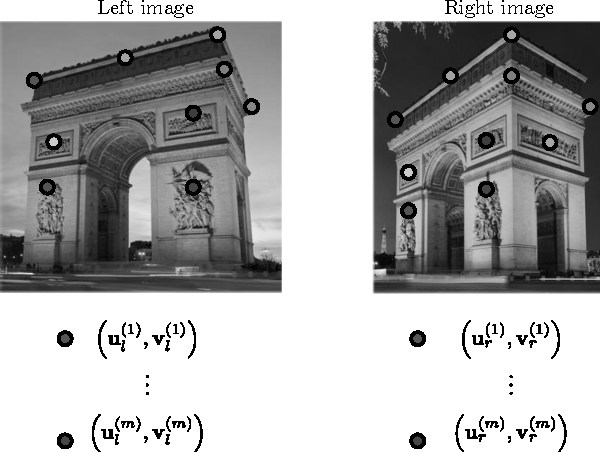
\includegraphics[width=0.5\columnwidth]{./images/features_matching.pdf}
    \end{center}

\end{frame}

\begin{frame}
    \frametitle{Stereo Calibration Procedure}
    
    Step A: For each correspondence $i$, write out epipolar constraint.

    \begin{equation*}
    \underbrace{\begin{bmatrix} u_l^{(i)} & v_l^{(i)} & 1 \end{bmatrix}}_{\text{Known}}
    \underbrace{\begin{bmatrix} f_{11} & f_{12} & f_{13} \\ f_{21} & f_{22} & f_{23} \\ f_{31} & f_{32} & f_{33} \end{bmatrix}}_{\text{Unknown}}
    \underbrace{\begin{bmatrix} u_r^{(i)} \\ v_r^{(i)} \\ 1 \end{bmatrix}}_{\text{Known}}
    = 0
    \end{equation*}

    Expand the matrix to get linear equation:

    \begin{equation*}
    (f_{11}u_r^{(i)} + f_{12}v_r^{(i)} + f_{13})u_l^{(i)} + (f_{21}u_r^{(i)} + f_{22}v_r^{(i)} + f_{23})v_l^{(i)} + f_{31}u_r^{(i)} + f_{32}v_r^{(i)} + f_{33} = 0
    \end{equation*}
    
\end{frame}

\begin{frame}
    \frametitle{Stereo Calibration Procedure}
    
    Step B: Rearrange terms to form a linear system.

    \begin{equation*}
        \underbrace{
        \begin{bmatrix}
            u_l^{(1)}u_r^{(1)} & u_l^{(1)}v_r^{(1)} & u_l^{(1)} & v_l^{(1)}u_r^{(1)} & v_l^{(1)}v_r^{(1)} & v_l^{(1)} & u_r^{(1)} & v_r^{(1)} & 1\\
            \vdots & \vdots & \vdots & \vdots & \vdots & \vdots & \vdots & \vdots & \vdots\\
            u_l^{(i)}u_r^{(i)} & u_l^{(i)}v_r^{(i)} & u_l^{(i)} & v_l^{(i)}u_r^{(i)} & v_l^{(i)}v_r^{(i)} & v_l^{(i)} & u_r^{(i)} & v_r^{(i)} & 1\\
            \vdots & \vdots & \vdots & \vdots & \vdots & \vdots & \vdots & \vdots & \vdots\\
            u_l^{(m)}u_r^{(m)} & u_l^{(m)}v_r^{(m)} & u_l^{(m)} & v_l^{(m)}u_r^{(m)} & v_l^{(m)}v_r^{(m)} & v_l^{(m)} & u_r^{(m)} & v_r^{(m)} & 1
        \end{bmatrix}}_{\substack{\vec{A}\\ \text{(Known)}}}
        \underbrace{\begin{bmatrix}
            f_{11} \\ f_{12} \\ f_{13} \\ f_{21} \\ f_{22} \\ f_{23} \\ f_{31} \\ f_{32} \\ f_{33}
        \end{bmatrix}}_{\substack{\vec{f}\\ \text{(Unknown)}}}
        =
        \begin{bmatrix}
            0 \\ \vdots \\ 0 \\ \vdots \\ 0
        \end{bmatrix}
    \end{equation*}

    \begin{center}
        \fbox{$\mathbf{A f = 0}$}
    \end{center}
    
\end{frame}

\begin{frame}
    \frametitle{The Tale of Missing Scale}
    
    Fundamental matrix acts on homogenous coordinates.

    \begin{equation*}
    \begin{bmatrix} u_l & v_l & 1 \end{bmatrix}
    \begin{bmatrix}
        f_{11} & f_{12} & f_{13} \\
        f_{21} & f_{22} & f_{23} \\
        f_{31} & f_{32} & f_{33}
    \end{bmatrix}
    \begin{bmatrix} u_r \\ v_r \\ 1 \end{bmatrix}
    = 0
    =
    \begin{bmatrix} u_l & v_l & 1 \end{bmatrix}
    \begin{bmatrix}
        kf_{11} & kf_{12} & kf_{13} \\
        kf_{21} & kf_{22} & kf_{23} \\
        kf_{31} & kf_{32} & kf_{33} \end{bmatrix}
    \begin{bmatrix} u_r \\ v_r \\ 1 \end{bmatrix}
    \end{equation*}

    Fundamental Matrix $\fundamentalMatrix$ and $k\fundamentalMatrix$ describe the same epipolar geometry. That is, $\fundamentalMatrix$ is defined only up to a scale.

    Set Fundamental Matrix to some arbitrary scale.

    \begin{center}
    \fbox{$||\fundamentalMatrix||^2 = 1$}
    \end{center}
    
\end{frame}

\begin{frame}
    \frametitle{Solving for $F$}
    
    Step C: Find least squares solution for fundamental matrix $F$.

    \vspace{0.5em} % Add some vertical space

    We want $\mathbf{A f}$ as close to 0 as possible and $||\mathbf{f}||^2 = 1$:

    \begin{center}
        \fbox{$\min_{\mathbf{f}} ||\mathbf{A f}||^2 \quad \text{such that} \quad ||\mathbf{f}||^2 = 1$}

        Constrained linear least squares problem
    \end{center}

    Like solving Projection Matrix during Camera Calibration. Or, Homography Matrix for Image Stitching.

    Rearrange solution $\mathbf{f}$ to form the fundamental matrix $\fundamentalMatrix$.
    
\end{frame}

\begin{frame}
    \frametitle{Extracting Rotation and Translation}
    
    Step D: Compute essential matrix $\essentialMatrix$ from known left and right intrinsic camera matrices and fundamental matrix $\fundamentalMatrix$.

    \begin{center}
        \fbox{$\essentialMatrix = \intrinsicMatrix_{l}^{\top} \fundamentalMatrix \intrinsicMatrix_{r}$}
    \end{center}

    Step E: Extract $\rotation$ and $\translation$ from $\essentialMatrix$.

    \begin{center}
        \fbox{$\essentialMatrix = \begin{bmatrix} \translation \end{bmatrix}_{\times} \rotation$}

        (Using Singular Value Decomposition)
    \end{center}

\end{frame}


\begin{frame}
    \frametitle{Geometría Epipolar}
    \footnotesize
    \begin{itemize}
        \item La restricción epipolar puede ser computada por medio de puntos 2D en la imagen cuando la pose relative de la cámara es conocida 
        ($\begin{bmatrix}
        \rotation & \translation
        \end{bmatrix}$), por ejemplo una cámara estéreo.
        \item El \textbf{plano epipolar} es definido por $\imagePoint_{l}$ y los dos centros óptico de las cámaras $\cameraCenter_{l}$ y $\cameraCenter_{r}$
        \item La \textbf{línea epipolar} es la intersección del plano epipolar y el plano de la imagen derecha.
        \item La restricción epipolar codifica que $\imagePoint_{r}$ debe estar ubicado sobre la linea epipolar en la imagen derecha.
    \end{itemize}

    \begin{center}
        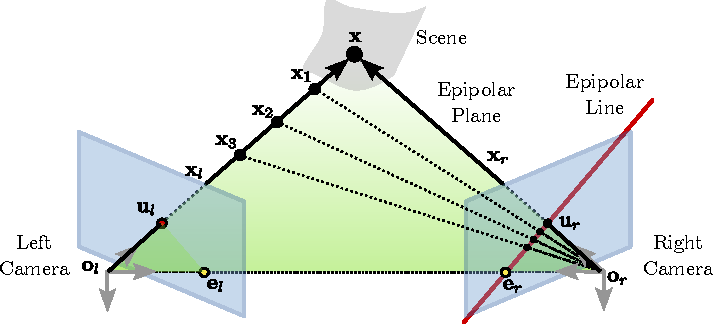
\includegraphics[width=0.6\textwidth]{./images/epipolar_geometry_epipolar_line.pdf}
    \end{center}

    La línea epipolar permite que restrinjamos la búsqueda de correspondencias visuales entre dos cámaras.

\end{frame}

\begin{frame}
    \frametitle{Finding Epipolar Lines}
    Given: Fundamental matrix $\mathbf{F}$ and point on left image $(u_l, v_l)$
    \vspace{0.2cm}
    Find: Equation of Epipolar line in the right image
    \vspace{0.2cm}
    Epipolar Constraint Equation:
    $$
    \begin{bmatrix} u_l & v_l & 1 \end{bmatrix}
    \begin{bmatrix}
        f_{11} & f_{12} & f_{13} \\
        f_{21} & f_{22} & f_{23} \\
        f_{31} & f_{32} & f_{33}
    \end{bmatrix}
    \begin{bmatrix} u_r \\ v_r \\ 1 \end{bmatrix} = 0
    $$

    Expanding the matrix equation gives:
    $$
    (f_{11} u_l + f_{21} v_l + f_{31}) u_r + (f_{12} u_l + f_{22} v_l + f_{32}) v_r + (f_{13} u_l + f_{23} v_l + f_{33}) = 0
    $$

    Equation for right epipolar line:
    $$\boxed{a_l u_r + b_l v_r + c_l = 0}$$

    Similarly we can calculate epipolar line in left image for a point in right image.
\end{frame}

\begin{frame}
    \frametitle{Finding Epipolar Lines: Example}
    
    \begin{columns}
        \begin{column}{0.45\textwidth} % Text column
            Given the Fundamental matrix,
            \begin{equation*}
                F = \begin{bmatrix}
                    -.003 & -.028 & 13.19 \\
                    -.003 & -.008 & -29.2 \\
                    2.97 & 56.38 & -9999
                \end{bmatrix}
            \end{equation*}
            and the left image point
            \begin{equation*}
                \vec{u}_l =
                \begin{bmatrix}
                    343 \\ 221 \\ 1
                \end{bmatrix}
            \end{equation*}
        \end{column}
        \begin{column}{0.55\textwidth} % Image column
            \centering
            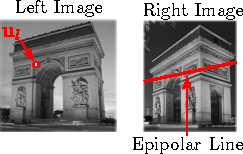
\includegraphics[width=0.8\textwidth]{./images/epipolar_line_example_1.pdf}
        \end{column}
    \end{columns}

    The equation for the epipolar line in the right image is
    \only<1>{
        \begin{equation*}
            \begin{bmatrix} u_r & v_r & 1 \end{bmatrix}
            \begin{bmatrix}
                -.003 & -.028 & 13.19 \\
                -.003 & -.008 & -29.2 \\
                2.97 & 56.38 & -9999
            \end{bmatrix}
            \begin{bmatrix}
                343 \\ 221 \\ 1
            \end{bmatrix} = 0
        \end{equation*}
    }
    \only<2>{
        \begin{equation*}
            0.03 u_r + 0.99 v_r - 265 = 0
        \end{equation*}
    }
\end{frame}

% --- Slide 13: Finding Correspondence (Search) ---
\begin{frame}
    \frametitle{Finding Correspondence}
    \centering

    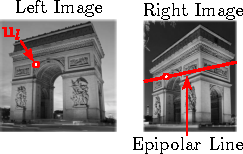
\includegraphics[width=0.5\textwidth]{./images/epipolar_line_example_2.pdf}
    
    Corresponding scene points lie on the epipolar lines.

    Finding correspondence is a 1D search.
\end{frame}

\begin{frame}
    \frametitle{Computing Depth}
    Given the intrinsic parameters, the projections of scene point $\mathbf{P}$ on the two image sensors are:
    \begin{equation*}
        \begin{bmatrix} u_l \\ v_l \\ 1 \end{bmatrix}
        \equiv
        \underbrace{\begin{bmatrix}
            f_x^{(l)} & 0 & o_x^{(l)} & 0 \\
            0 & f_y^{(l)} & o_y^{(l)} & 0 \\
            0 & 0 & 1 & 0
        \end{bmatrix}}_{\mathbf{P}}
        \begin{bmatrix} x_l \\ y_l \\ z_l \\ 1 \end{bmatrix}
    \end{equation*}
    \begin{equation*}
        \begin{bmatrix} u_r \\ v_r \\ 1 \end{bmatrix}
        \equiv
        \underbrace{\begin{bmatrix}
            f_x^{(r)} & 0 & o_x^{(r)} & 0 \\
            0 & f_y^{(r)} & o_y^{(r)} & 0 \\
            0 & 0 & 1 & 0
        \end{bmatrix}}_{\mathbf{M}}
        \begin{bmatrix} x_r \\ y_r \\ z_r \\ 1 \end{bmatrix}
    \end{equation*}
\end{frame}

% --- Slide 15: Computing Depth (Transformation) ---
\begin{frame}
    \frametitle{Computing Depth}
    Left Camera Imaging Equation
    $$
    \begin{bmatrix} u_l \\ v_l \\ 1 \end{bmatrix} \equiv
    \begin{bmatrix}
        f_x^{(l)} & 0 & o_x^{(l)} \\
        0 & f_y^{(l)} & o_y^{(l)} \\
        0 & 0 & 1
    \end{bmatrix}
    \begin{bmatrix} x_l \\ y_l \\ z_l \end{bmatrix}
    $$
    Right Camera Imaging Equation
    $$
    \begin{bmatrix} u_r \\ v_r \\ 1 \end{bmatrix} \equiv
    \begin{bmatrix}
        f_x^{(r)} & 0 & o_x^{(r)} \\
        0 & f_y^{(r)} & o_y^{(r)} \\
        0 & 0 & 1
    \end{bmatrix}
    \begin{bmatrix} x_r \\ y_r \\ z_r \end{bmatrix}
    $$

    We also know the relative position and orientation between the two cameras.
    $$
    \begin{bmatrix} x_l \\ y_l \\ z_l \\ 1 \end{bmatrix} =
    \begin{bmatrix}
        r_{11} & r_{12} & r_{13} & t_x \\
        r_{21} & r_{22} & r_{23} & t_y \\
        r_{31} & r_{32} & r_{33} & t_z \\
        0 & 0 & 0 & 1
    \end{bmatrix}
    \begin{bmatrix} x_r \\ y_r \\ z_r \\ 1 \end{bmatrix}
    $$
\end{frame}

% --- Slide 16: Computing Depth (Combined Equations) ---
\begin{frame}
    \frametitle{Computing Depth}
    Left Camera Imaging Equation:
    $$
    \begin{bmatrix} u_l \\ v_l \\ 1 \end{bmatrix} \equiv
    \begin{bmatrix}
        f_x^{(l)} & 0 & o_x^{(l)} & 0 \\
        0 & f_y^{(l)} & o_y^{(l)} & 0 \\
        0 & 0 & 1 & 0
    \end{bmatrix}
    \begin{bmatrix}
        r_{11} & r_{12} & r_{13} & t_x \\
        r_{21} & r_{22} & r_{23} & t_y \\
        r_{31} & r_{32} & r_{33} & t_z \\
        0 & 0 & 0 & 1
    \end{bmatrix}
    \begin{bmatrix} x_r \\ y_r \\ z_r \\ 1 \end{bmatrix}
    $$
    $$\boxed{\vec{u}_l \equiv \mathbf{P}_l \tilde{\mathbf{x}}_r}$$

    Right Camera Imaging Equation:
    $$
    \begin{bmatrix} u_r \\ v_r \\ 1 \end{bmatrix} \equiv
    \begin{bmatrix}
        f_x^{(r)} & 0 & o_x^{(r)} & 0 \\
        0 & f_y^{(r)} & o_y^{(r)} & 0 \\
        0 & 0 & 1 & 0
    \end{bmatrix}
    \begin{bmatrix} x_r \\ y_r \\ z_r \\ 1 \end{bmatrix}
    $$
    $$\boxed{\vec{u}_r \equiv \mathbf{M}_{\text{int}} \tilde{\mathbf{x}}_r}$$
\end{frame}

% --- Slide 17: Computing Depth (Matrix Equations) ---
\begin{frame}
    \frametitle{Computing Depth}
    The imaging equations:
    $$
    \vec{u}_r \propto
    \underbrace{\begin{bmatrix}
        m_{11} & m_{12} & m_{13} & m_{14} \\
        m_{21} & m_{22} & m_{23} & m_{24} \\
        m_{31} & m_{32} & m_{33} & m_{34}
    \end{bmatrix}}_{\text{Known}}
    \underbrace{\begin{bmatrix} x_r \\ y_r \\ z_r \\ 1 \end{bmatrix}}_{\text{Unknown}}
    \quad \vec{u}_r = \mathbf{M}_r \tilde{\mathbf{x}}_r
    $$
    $$
    \vec{u}_l \propto
    \underbrace{\begin{bmatrix}
        p_{11} & p_{12} & p_{13} & p_{14} \\
        p_{21} & p_{22} & p_{23} & p_{24} \\
        p_{31} & p_{32} & p_{33} & p_{34}
    \end{bmatrix}}_{\text{Known}}
    \underbrace{\begin{bmatrix} x_r \\ y_r \\ z_r \\ 1 \end{bmatrix}}_{\text{Unknown}}
    \quad \vec{u}_l = \mathbf{P}_l \tilde{\mathbf{x}}_r
    $$

    Rearranging the terms:
    $$
    \begin{bmatrix}
        u_r m_{31} - m_{11} & u_r m_{32} - m_{12} & u_r m_{33} - m_{13} \\
        v_r m_{31} - m_{21} & v_r m_{32} - m_{22} & v_r m_{33} - m_{23} \\
        u_l p_{31} - p_{11} & u_l p_{32} - p_{12} & u_l p_{33} - p_{13} \\
        v_l p_{31} - p_{21} & v_l p_{32} - p_{22} & v_l p_{33} - p_{23}
    \end{bmatrix}
    \begin{bmatrix} x_r \\ y_r \\ z_r \end{bmatrix} =
    \begin{bmatrix}
        m_{14} - u_r m_{34} \\
        m_{24} - v_r m_{34} \\
        p_{14} - u_l p_{34} \\
        p_{24} - v_l p_{34}
    \end{bmatrix}
    $$
\end{frame}

% --- Slide 18: Computing Depth (Least Squares) ---
\begin{frame}
    \frametitle{Computing Depth: Least Squares Solution}
    $$
    \underbrace{\begin{bmatrix}
        u_r m_{31} - m_{11} & u_r m_{32} - m_{12} & u_r m_{33} - m_{13} \\
        v_r m_{31} - m_{21} & v_r m_{32} - m_{22} & v_r m_{33} - m_{23} \\
        u_l p_{31} - p_{11} & u_l p_{32} - p_{12} & u_l p_{33} - p_{13} \\
        v_l p_{31} - p_{21} & v_l p_{32} - p_{22} & v_l p_{33} - p_{23}
    \end{bmatrix}}_{\mathbf{A}_{4\times3} \text{(Known)}}
    \underbrace{\begin{bmatrix} x_r \\ y_r \\ z_r \end{bmatrix}}_{\mathbf{x}_r \text{(Unknown)}} =
    \underbrace{\begin{bmatrix}
        m_{14} - u_r m_{34} \\
        m_{24} - v_r m_{34} \\
        p_{14} - u_l p_{34} \\
        p_{24} - v_l p_{34}
    \end{bmatrix}}_{\mathbf{b}_{4\times1} \text{(Known)}}
    $$

    Find least squares solution using pseudo-inverse:
    $$
    \mathbf{A} \mathbf{x}_r = \mathbf{b}
    $$
    $$
    \mathbf{A}^T \mathbf{A} \mathbf{x}_r = \mathbf{A}^T \mathbf{b}
    $$
    $$
    \boxed{\mathbf{x}_r = (\mathbf{A}^T \mathbf{A})^{-1} \mathbf{A}^T \mathbf{b}}
    $$
\end{frame}


\begin{frame}
    \frametitle{Matríz Esencial}
    \footnotesize

    La {\bf Matríz Esencial} es una especialización de la {\bf Matríz Fundamental}. La Matríz Esencial trabaja sobre {\bf coordenadas  normalizadas}  de la imagen, es decir, requiere conocer la calibración de las cámaras, mientras que la Matríz Fundamental relaciona correspondencias desconociendo las calibraciones.

    \begin{block}{Coordenadas Normalizadas:}
        Dado $\homoImagePoint = \projectionMatrix \homoWorldPoint$, con $\projectionMatrix = \intrinsicMatrix [\rotation|\translation]$, si conocemos la matríz de calibración $\intrinsicMatrix$ entonces $\hat{\imagePoint} = \inverse{\intrinsicMatrix} \homoImagePoint$ decimos que $\hat{\imagePoint}$ está en {\bf coordenadas normalizadas}. Se lo puede pensar como una imagen del punto $\homoWorldPoint$ con respecto a una cámara $[\rotation|\translation]$ teniendo la matriz de calibración como la identidad. $ \inverse{\intrinsicMatrix} \projectionMatrix = [\rotation| \translation]$ se denomina {\bf cámara normalizada} donde los parámetros de calibración han sido removidos.
    \end{block}
%
    \begin{equation*}
        \hat{\imagePoint}^{\prime\top} \essentialMatrix \hat{\imagePoint}  = 0 \quad \text{(restricción de coplanaridad)}
    \end{equation*}
    donde $\essentialMatrix = \begin{bmatrix}
        \translation 
    \end{bmatrix}_{\times} \rotation$, y se denomina \emph{Essential Matrix}.
%
    \begin{align*}
        \hat{\imagePoint}^{\prime\top} \essentialMatrix \hat{\imagePoint}  &= 0\\
        \left( \inverse{\intrinsicMatrix^{\prime}} \homoImagePoint^{\prime} \right)^{\top} \essentialMatrix \left( \inverse{\intrinsicMatrix} \homoImagePoint \right) &= 0\\
        \homoImagePoint^{\prime\top} \inverse{\intrinsicMatrix^{\prime\top}} \essentialMatrix \inverse{\intrinsicMatrix} \homoImagePoint&= 0
    \end{align*}
    La relación entre la matriz fundamental y la matríz esencial está dada por
    \begin{equation*}
        \essentialMatrix = \intrinsicMatrix^{\prime\top} \fundamentalMatrix \intrinsicMatrix
    \end{equation*}

    \note{has only five degrees of freedom: both the rotation matrix R and the translation t have three degrees of freedom, but there is an overall scale ambiguity - like the fundamental matrix, the essential matrix is a homogeneous quantity.}
    
\end{frame}

\begin{frame}
    \frametitle{Matríz Esencial}

    \note{Info: https://3d.bk.tudelft.nl/courses/geo1016/slides/Lecture_05_Reconstruct3DGeometry.pdf}

    El plan es que podamos computar la Matríz Fundamental, y luego utilizando la calibración de la cámara calcular la Matríz Esencial. La Matríz Esencial está compuesta por rotación entre las cámaras y el vector dirección de traslación (a un factor de escala).
    
    \begin{figure}
        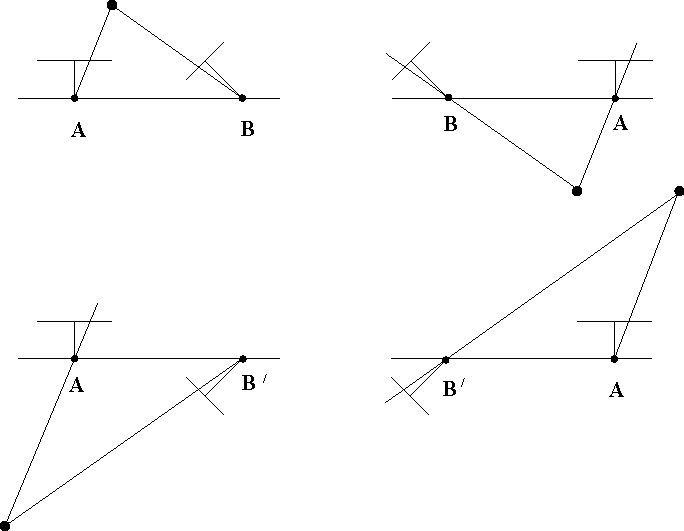
\includegraphics[width=0.4\textwidth]{./images/essential_matrix_possible_solutions.pdf}
    \end{figure}

    En total tenemos 4 configuraciones posibles para las 2 cámaras. Nos quedamos con la configuración que haga que los puntos triangulados esten delante de ambas cámaras.
\end{frame}


\begin{frame}
    \frametitle{Matríz Fundamental vs Matríz Esencial}
    \footnotesize
    \note{Ver vídeo de clase de Staschnis https://youtu.be/auhpPoAqprk}
    
    \begin{itemize}
        \item Ambas matrizes tienen rango 2
        \item La matríz esencial tiene 5 DoF
        \item La matríz fundamental tiene 7 DoF (ya que contiene información sobre los parámetros de calibración)
        \item Las restricciones coplanares más pares de correspondencias nos permiten encontrar dichas matrices por medio de la solución de un sistema líneal utilizando descomposición SVD (\emph{Singular Value Decomposition}).
        \item La matríz fundamental puede ser hallada con \emph{8-Point Algorithm}
        \item La matríz esencial puede ser hallada con \emph{5-Point Algorithm}
        \item Una vez obtenida la matríz esencial podemos obtener la rotación y traslación (con ambig{\"u}edad de escala)
        \item La matríz esencial o fundamental nos permiten delimitar la búsqueda de correspondencias en las líneas epipolares únicamente, en vez de tener que buscar en toda la imagen.
    \end{itemize}

    \begin{figure}
        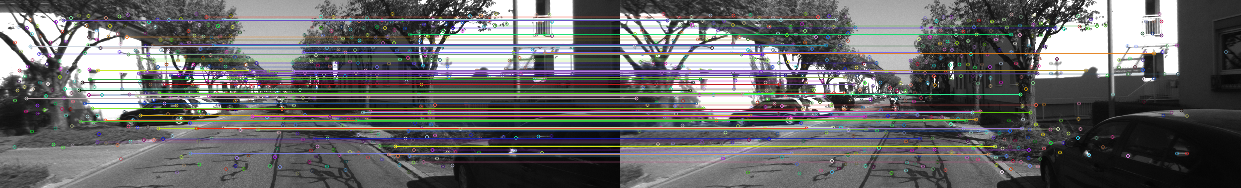
\includegraphics[width=\textwidth]{./images/stereo_matches.pdf}
    \end{figure}
    
\end{frame}


\begin{frame}
    \frametitle{Triangulación estéreo (con cámara rectificada)}
    \footnotesize
    \begin{figure}
        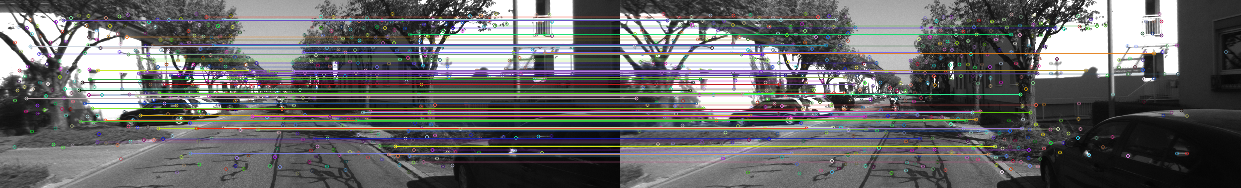
\includegraphics[width=0.5\textwidth]{./images/stereo_matches.pdf}
        \caption{Matching estéreo.}    
    \end{figure}
    \vspace{-2em}
    \begin{minipage}[t]{0.65\textwidth}
        \begin{figure}
            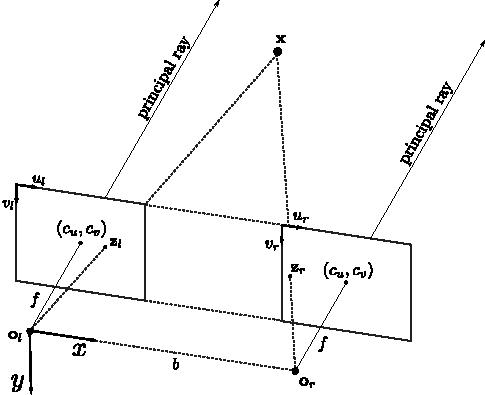
\includegraphics[width=0.65\textwidth]{./images/stereo_triangulation.pdf}
        \end{figure}
    \end{minipage}
    \begin{minipage}[t]{0.3\textwidth}
        \centering
        \begin{align*}
            \point&=\begin{bmatrix}x & y & z\end{bmatrix}^{\top}\\
            x &= \frac{(u_{l}-c_{u})z}{f}\\
            y &= \frac{(v_{l}-c_{v})z}{f}\\
            z &= \frac{bf}{u_{l}-u_{r}}
        \end{align*}
    \end{minipage}
    \centering
    
    Triangulación estéreo.
\end{frame}

\begin{frame}
    \frametitle{Triangulación estéreo (con cámara rectificada)}
    
    \begin{figure}[!htb]
        \centering
        \subfloat[]
        {
            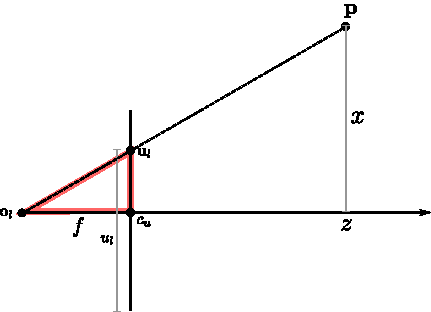
\includegraphics[width=0.35\columnwidth]{./images/stereo_triangulation2.pdf}
        }
        \hspace{1em}
        \subfloat[]
        {
            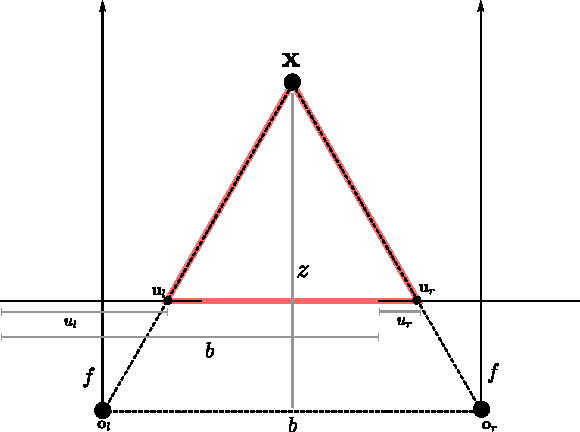
\includegraphics[width=0.45\columnwidth]{./images/stereo_triangulation3.pdf}
        }\\
        \subfloat[]
        {
            \includegraphics[width=0.7\columnwidth]{./images/depth_disparity_equation.pdf}
        }
    \end{figure}
    
    % \begin{equation*}
    %     \frac{b}{z} = \frac{b - (\imagePoint_{l} - \imagePoint_{r})}{z-f} \Rightarrow z = \frac{fb}{(\imagePoint_{l} - \imagePoint_{r})}  = \frac{fb}{d}
    % \end{equation*}
    
\end{frame}

\begin{frame}
    \frametitle{Disparidad}
    \footnotesize
    \begin{figure}[!h]
        \includegraphics[width=0.6\textwidth]{images/disparity.pdf}
    \end{figure}

    Ejemplo de disparidad: pongamos un dedo enfrente de nuestros ojos a una distancia \SI{20}{\centi\meter} y alternadamente cerremos y abramos cada ojo.
\end{frame}

\begin{frame}
    \frametitle{Stereo Matching: Finding Disparities}
    \note{https://youtu.be/hUVyDabn1Mg}
    \begin{center}
        \only<1>{\includegraphics[width=\textwidth]{images/block_matching_disparity_1.pdf}}

        \only<2>{\includegraphics[width=\textwidth]{images/block_matching_disparity_2.pdf}}

        \only<3>{\includegraphics[width=\textwidth]{images/block_matching_disparity_3.pdf}}
        
        \only<4>{\includegraphics[width=\textwidth]{images/block_matching_disparity_4.pdf}}

        \only<5>{\includegraphics[width=\textwidth]{images/block_matching_disparity_5.pdf}}
    \end{center}

\end{frame}


\begin{frame}
    \frametitle{Similarity Metrics for Template Matching}
    \note{https://youtu.be/hUVyDabn1Mg}
    \begin{itemize}
        \item Find pixel $(k, l) \in L$ with Minimum Sum of Absolute Differences (SAD):
        \begin{equation*}
            \text{SAD}(k, l) = \sum_{(i, j) \in T} |E_t(i, j) - E_r(i + k, j + l)|
        \end{equation*}

        \item Find pixel $(k, l) \in L$ with Minimum Sum of Squared Differences (SSD):
        \begin{equation*}
            \text{SSD}(k, l) = \sum_{(i, j) \in T} |E_t(i, j) - E_r(i + k, j + l)|^2
        \end{equation*}

        \item Find pixel $(k, l) \in L$ with Maximum Normalized Cross-Correlation (NCC):
        \begin{equation*}
            \text{NCC}(k, l) = \frac{\sum_{(i, j) \in T} E_t(i, j) E_r(i + k, j + l)}{\sqrt{\sum_{(i, j) \in T} E_t(i, j)^2 \sum_{(i, j) \in T} E_r(i + k, j + l)^2}}
        \end{equation*}
    \end{itemize}
\end{frame}


\begin{frame}
    \frametitle{Examples of disparity maps}
    \note{https://youtu.be/hUVyDabn1Mg}
    \begin{figure}[!htb]
        \centering
        \subfloat[Window size = 5 pixels (Sensitive to noise)]
        {
            \includegraphics[width=0.45\columnwidth]{./images/tsukuba_disparity_map_5x5_window.png}
        }
        \hspace{1em}
        \subfloat[Window size = 30 pixels (Poor localization)]
        {
            \includegraphics[width=0.45\columnwidth]{./images/tsukuba_disparity_map_30x30_window.png}
        }
    \end{figure}

\end{frame}

\begin{frame}
    \frametitle{Estimación de movimiento}
    \scriptsize
    \note{imagenes extraidas de https://vision.in.tum.de/_media/teaching/ss2020/visnav_ss2020/visnav_lecture3.pdf}
    
    \underline{\textbf{2D-2D}}
    
    \begin{columns}
        \begin{column}{0.7\textwidth}
            \begin{itemize}
            \item Error de reproyección:
            \begin{center}
                $f(\transform{a}{b}, \mapPointsSet)= \sum_{i=1}^{N} \Vert \measurement_{a,i} - \prediction^{\mathrm{s}}(\transform{a}{\worldCoordSystem},\worldPoint_{i}) \Vert^{2} + \Vert \measurement_{b,i} - \prediction^{\mathrm{s}}(\inverse{\transform{a}{b}}\transform{a}{\worldCoordSystem},\worldPoint_{i}) \Vert^{2}$
            \end{center}
            \item Algoritmos lineales: 8-point, 5-point
            \end{itemize}
        \end{column}
        \begin{column}{0.3\textwidth}
            \begin{figure}
                \includegraphics[width=0.5\columnwidth]{./images/localization_2d_2d.pdf}
            \end{figure}
        \end{column}
    \end{columns}

    \underline{\textbf{3D-2D}}
    \begin{columns}
    \begin{column}{0.7\textwidth}
        \begin{itemize}
            \item Error de reproyección:
            \begin{center}
                $f(\transform{\worldCoordSystem}{a})= \sum_{i=1}^{N} \Vert \measurement_{a,i} - \prediction(\inverse{\transform{\worldCoordSystem}{a}},\worldPoint_{i}) \Vert^{2}$
            \end{center}
            \item Algoritmos lineales: DLT, PnP
        \end{itemize}
    \end{column}
    \begin{column}{0.3\textwidth}
        \begin{figure}
            \includegraphics[width=0.5\columnwidth]{./images/localization_3d_2d.pdf}
        \end{figure}
    \end{column}
    \end{columns}
    \underline{\textbf{3D-3D}}
    \begin{columns}
        \begin{column}{0.7\textwidth}
            \begin{itemize}
                \item Error de reproyección:
                \begin{center}
                    $f(\transform{a}{b})= \sum_{i=1}^{N} \Vert \pointCoord{a}_{i} - \transform{a}{b} \pointCoord{b}_{i} \Vert^{2}$
                \end{center}
                \item Algoritmos lineales: Atun, Horn
            \end{itemize}
        \end{column}
        \begin{column}{0.3\textwidth}
            \begin{figure}
                \includegraphics[width=0.4\columnwidth]{./images/localization_3d_3d.pdf}
            \end{figure}
        \end{column}
    \end{columns}

\end{frame}

\begin{frame}
    \frametitle{Estimación de movimiento 2D-2D}
    \footnotesize
    
    \begin{itemize}
        \item Dados matches 2D-2D $\{(\measurement_{a}, \measurement_{b})_{i}\}$ de puntos 3D desconocidos $\mapPointsSet_{i}$ encontrar el movimiento relativo $\transform{a}{b}$ entre los frames.
        \item Error de reproyección (Bundle Adjustment):
        \[
        f(\transform{a}{b}, \mapPointsSet)= \sum_{i=1}^{N} \Vert \measurement_{a,i} - \prediction^{\mathrm{s}}(\transform{a}{\worldCoordSystem},\worldPoint_{i}) \Vert^{2} + \Vert \measurement_{b,i} - \prediction^{\mathrm{s}}(\inverse{\transform{a}{b}}\transform{a}{\worldCoordSystem},\worldPoint_{i}) \Vert^{2}
        \]
        Se puede optimizar con métodos no lineales pero requieren de una buena semilla inicial. Es no convexo, solución no única (ambigüedadad de escala)
        \item Se puede utilizar un enfoque algebraico basado en geometría epipolar para obtener la transformación relativa (a un factor de escala) sin explicitamente computar la posición de los puntos 3D: algoritmos 8-point y 5-point.
        \item Aplicaciones:
        \begin{itemize}
            \item Filtrar matches con RANSAC
            \item Inicializar una sistemas de SLAM monocular / SfM
        \end{itemize}
    \end{itemize}
\end{frame}

\begin{frame}
    \frametitle{Estimación de movimiento 3D-2D}
    \footnotesize
    
    \begin{itemize}
        \item Dado un conjunto de correspondencias 3D-2D $\{(\worldPoint, \measurement_{a})_{i}\}$ queremos encontrar la pose $\transform{w}{a}$ de la cámara en el mundo.
        \item Error de reproyección:
        \[
        f(\transform{\worldCoordSystem}{a})= \sum_{i=1}^{N} \Vert \measurement_{a,i} - \prediction(\inverse{\transform{\worldCoordSystem}{a}},\worldPoint_{i}) \Vert^{2}
        \]
        Se puede optimizar con métodos no lineales pero requieren de una buena semilla inicial. Es no convexo, solución no única (ambigüedad de escala)
        \item Este problema es conocido como \emph{Perspective-n-Points} (PnP) y existen diferentes enfoques para resolverlo:
        \begin{itemize}
            \item Direct Linear Transform (DLT)
            \item EPnP
            \item OPnP
        \end{itemize}
        \item Aplicaciones:
        \begin{itemize}
            \item Localización de una cámara dado un mapa de puntos (tracking)
        \end{itemize}
    \end{itemize}
    
\end{frame}

\begin{frame}
    \frametitle{Matching 3D-2D}
    
    \begin{figure}
        \includegraphics{./images/tracking_reprojection_error_before.pdf}
    \end{figure}
    
    \note{Ejemplo de trackeo de 3 puntos del mapa.\\
        
        Imaginemos que estamos en el segundo frame estéreo y ya tenemos el mapa inicial reconstruido por el primer frame estéreo dado por la cámara.\\
        
        Los puntos del mapa son proyectados sobre los planos de las imagenes de la cámara izquierda y derecha, y se buscan las correspondencias entre el punto del mapa y los features extraidos en las imagenes mediante la comparación de los descriptores.\\
        
        Para limitar la busqueda de correspondencias, se divide la imagen en celdas y se busca los candidatos a ser matcheados en celdas vecinas a la celda donde cae cada proyeccion.}
    
\end{frame}

\begin{frame}
    \frametitle{Ajuste de pose}
    
    \begin{figure}
        \includegraphics{./images/tracking_reprojection_error_after.pdf}
    \end{figure}
    \note{
        Correccion de los errores de proyeccion.\\
        Observar que la camara derecha esta fija con respecto a la camara izquierda.}
\end{frame}

\begin{frame}
    \frametitle{Local Bundle Adjustment}
    
    \begin{figure}
        \includegraphics[width=\textwidth]{./images/ba_reprojection_error_before.pdf}
    \end{figure}
    
    \note{Ejemplo de ajuste de 3 keyframes que ven 2 puntos del mapa.\\
        k1 - x1 medición estéreo\\
        k1 - x2 medición derecha\\
        k2 - x1 medición estéreo\\
        k2 - x2 medición estéreo\\
        k3 - x1 medición izquierda\\
        k3 - x2 medición estéreo}
    
\end{frame}

\begin{frame}
    \frametitle{Local Bundle Adjustment}
    
    \begin{figure}
        \includegraphics[width=\textwidth]{./images/ba_reprojection_error_after.pdf}
    \end{figure}
    
    \note{Ajustamos los keyframes y los puntos!!!\\
        Una ecuación de error por cada medición (6 en total).\\
        Nuevamente tenemos en cuenta la transformación rígida entre la cámara izquierda y la cámara derecha para las mediciones derechas.}
    
\end{frame}


\begin{frame}
    \frametitle{Estimación de movimiento 3D-3D}
    \footnotesize
    
    \begin{itemize}
        \item Dado un conjunto de correspondencias 3D en dos sistemas de coordenadas distintos: $\{(\pointCoord{a}, \pointCoord{b})_{i}\}$ queremos encontrar la transformación relativa $\transform{a}{b}$.
        \item Error geométrico 3D:
        \[
        f(\transform{a}{b})= \sum_{i=1}^{N} \Vert \pointCoord{a}_{i} - \transform{a}{b} \pointCoord{b}_{i} \Vert^{2}
        \]
        Corresponde a alineamiento de nube de puntos por mínimos cuadrados.
        \item Solución cerrada, eg.g Arun et al, 1987
        \item Aplicaciones:
        \begin{itemize}
            \item Obtención de movimiento relativo para cámaras estéreo (mediante el uso de puntos triangulados) o RGB-D (mediciones con profundidad)
            \item Corrección de Loop Closure (variante con estimación de escala para SLAM monocular)
        \end{itemize}
    \end{itemize}
    
\end{frame}

\begin{frame}
    \frametitle{Tipos de transformaciones 2D}
    \footnotesize
    
    \begin{figure}
        \includegraphics[width=0.9\columnwidth]{./images/transformation_table_2d.pdf}
    \end{figure}
    
\end{frame}

\begin{frame}
    \frametitle{Tipos de transformaciones 2D}

    \TODO{mejorar esta slides con \url{https://rpg.ifi.uzh.ch/docs/teaching/2020/11_tracking.pdf}}
    
\end{frame}


\begin{frame}
    \frametitle{Tipos de transformaciones 3D}
    \footnotesize
    
    \begin{figure}
        \includegraphics[width=0.6\columnwidth]{./images/transformation_table_3d.pdf}
    \end{figure}
    
\end{frame}


\begin{frame}<presentation:0>[noframenumbering]
    \frametitle{Direct Linear Transformation (DLT) algorithm}
    \footnotesize
    \TODO{Book Multiview Geometry: 4.1 The Direct Linear Transformation (DLT) algorithm}
    
\end{frame}
